\chapter{Impact}
\label{ch:impact}

\section{Introduction}

This chapter details the impact such as the work described in this thesis has had, including outcomes like artworks that were made by myself and others; and recognition, such as exhibitions and awards. 
This also includes an overview of work and research that follows and has been influenced by this research, applications of the research into other domains, and examples of ideas from this thesis being used and put into technologies and practical interfaces. 

\section{\textit{(un)stable equilibrium}}
\label{c7:sec:unstable_eq}

As a direct outcome of the experiments detailed in Chapter \ref{ch:unstable_eq}, a series of six video artworks titled \textit{(un)stable equilibrium 1:1, 1:2, … 1:6} were made by sampling from the paired generative models, in-parallel, using the same latent code  (Fig. \ref{fig:c7:ue_still}). 
A looping (spherical) latent space interpolation \citep{white2016sampling} of the two videos was produced, which lasted approximately one hour. 
The interpolations were deliberately designed to be slow to provide a meditative loop seamlessly so that it could be played in a gallery setting without any interruption.

\begin{figure}[!htb]
    \centering
    \captionsetup{justification=centering}
    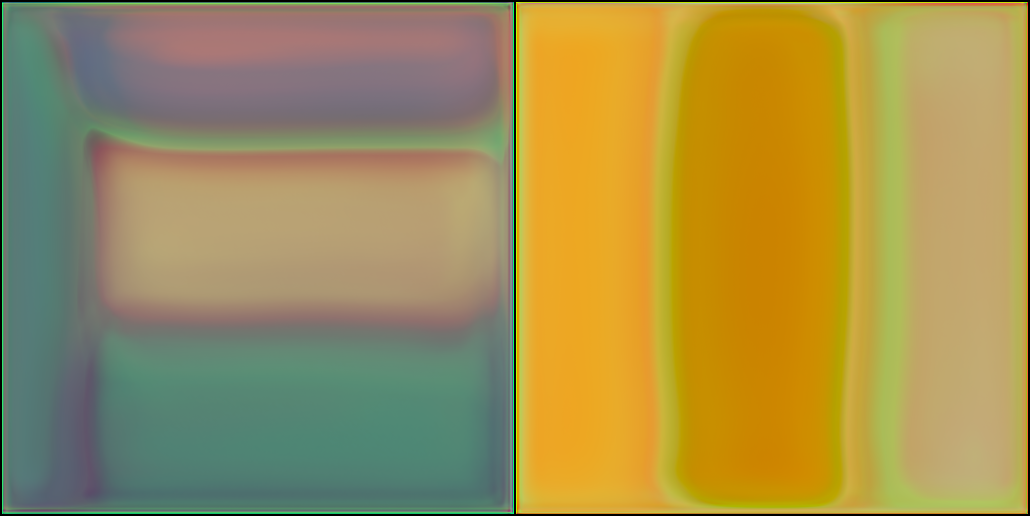
\includegraphics[width=1\textwidth]{figures/c7_impact/ue_1_1_still.png}
    \caption{Still from \textit{(un)stable equilibrium 1:1}.}
    \label{fig:c7:ue_still}
\end{figure}

The works were first shown in the exhibitions for the respective conferences ICCV (International Conference on Computer Vision) and NeurIPS (Conference on Neural Information Processing Systems) in 2019. 
At NeurIPS the works were shown in the AI Art Gallery, where the work was also presented as a workshop presentation at the NeurIPS Workshop for Creativity and Design. 
At ICCV the work was shown in the Computer Vision Art Gallery, where it won the Grand Prize in Computer Vision Art, an honour that is only shared between myself \citep{broad2019unstable}, Anna \citet{ridler2018mosaic} and Nouf \citet{aljowaysir2021salaf}.

The work was shown in a gallery setting in March 2020 in Geneva, Switzerland at One Gee in Fog, though unfortunately, that exhibition had to be cut short after 2 days because of the imposition of the COVID lockdown in Switzerland. 
In lockdown, I began producing prints of the works onto metal aluminium plates, where the glossy finish was a good match for the highly saturated colours in many of the prints. 
Initially, I was selling these prints online through my own website. Physical works in this series were later exhibited and sold in the commercial London gallery \textit{the depot\_}, in their debut show titled \textit{the depot\_ digs} \citep{depot2021digs}  (Fig. \ref{fig:c7:depot_digs}), where I was also invited to give an artists talk in 2021.

\begin{figure}[!htb]
    \centering
    \captionsetup{justification=centering}
    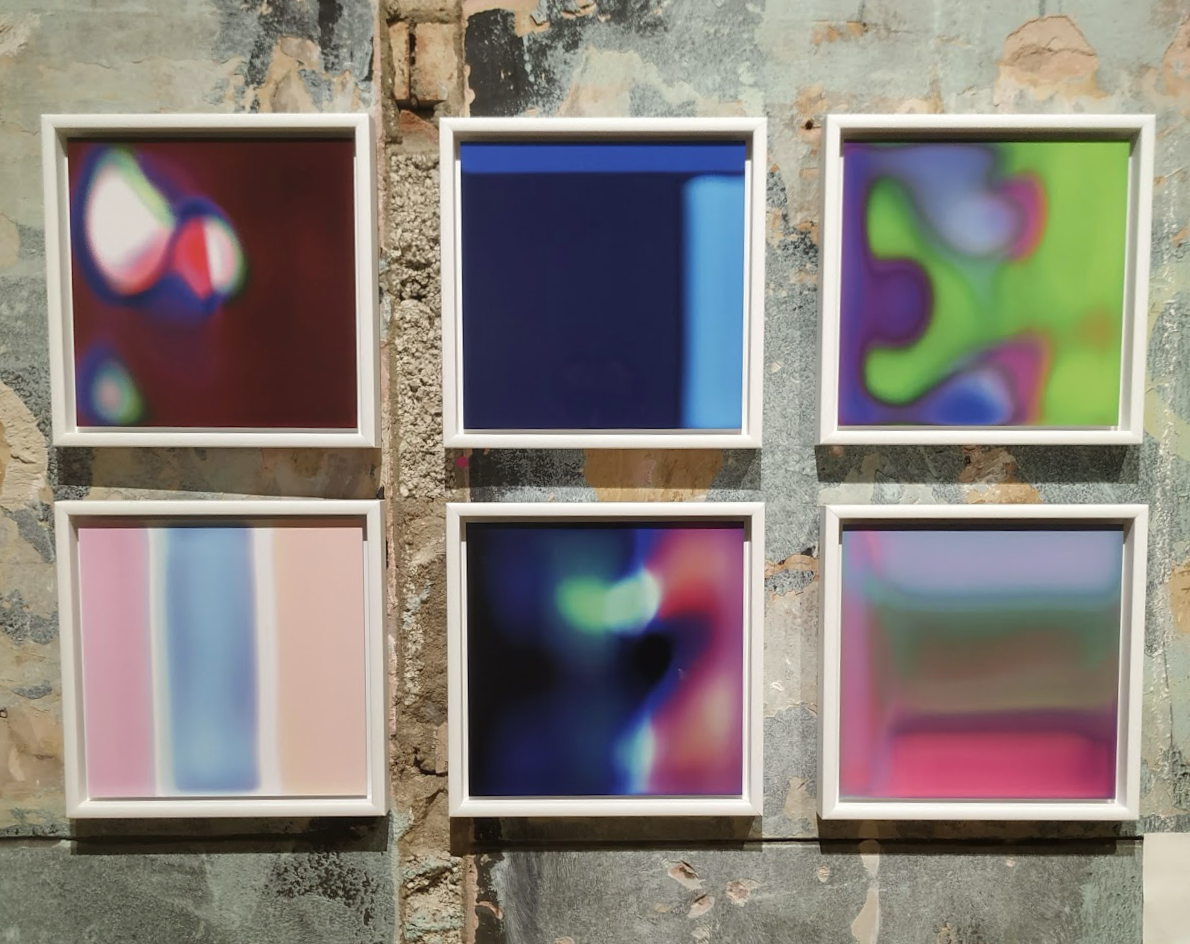
\includegraphics[width=1\textwidth]{figures/c7_impact/depot_cropped.png}
    \caption[Installation shot of \textit{(un)stable equilibrium} in the depot\_ gallery]{Installation shot of \textit{(un)stable equilibrium} prints in \textit{the depot\_ digs} exhibition at the depot\_ gallery in London (2021).}
    \label{fig:c7:depot_digs}
\end{figure}

Following the COVID-19 pandemic, the original video work \textit{(un)stable equilibrium 1:1} was shown at the FILE festival. 
File Festival is the premier digital arts festival in South America, where the work was installed in the Fiesp Cultural Centre in São Paolo. 
Here, the work was presented in its originally intended form as a lopping video piece in a gallery installation setting  (Fig. \ref{fig:c7:file-festival}).

\begin{figure}[!htb]
    \centering
    \captionsetup{justification=centering}
    \includegraphics[width=1\textwidth]{figures/c7_impact/FILE-festival.png}
    \caption[Installation shot of \textit{(un)stable equilibrium} at FILE festival]{Installation shot of \textit{(un)stable equilibrium 1:1} at \textit{FILE Festival} in the Centro Cultural Fiesp, São Paolo (2022). Image courtesy of FILE - Electronic Language International Festival (permission to reproduce TBC).}
    \label{fig:c7:file-festival}
\end{figure}

\section{Divergent fine-tuning}
\label{c7:sec:divergent}


Directly from the latter set of experiments described in Chapter \ref{ch:divergent}, inverting the objective function, the series of artworks \textit{Being Foiled}  (Fig. \ref{fig:c7:being-foiled}), were produced using the model checkpoints after 500 iterations from the 512x512 StyleGAN FFHQ model. 

\begin{figure}[!htb]
    \centering
    \captionsetup{justification=centering}
    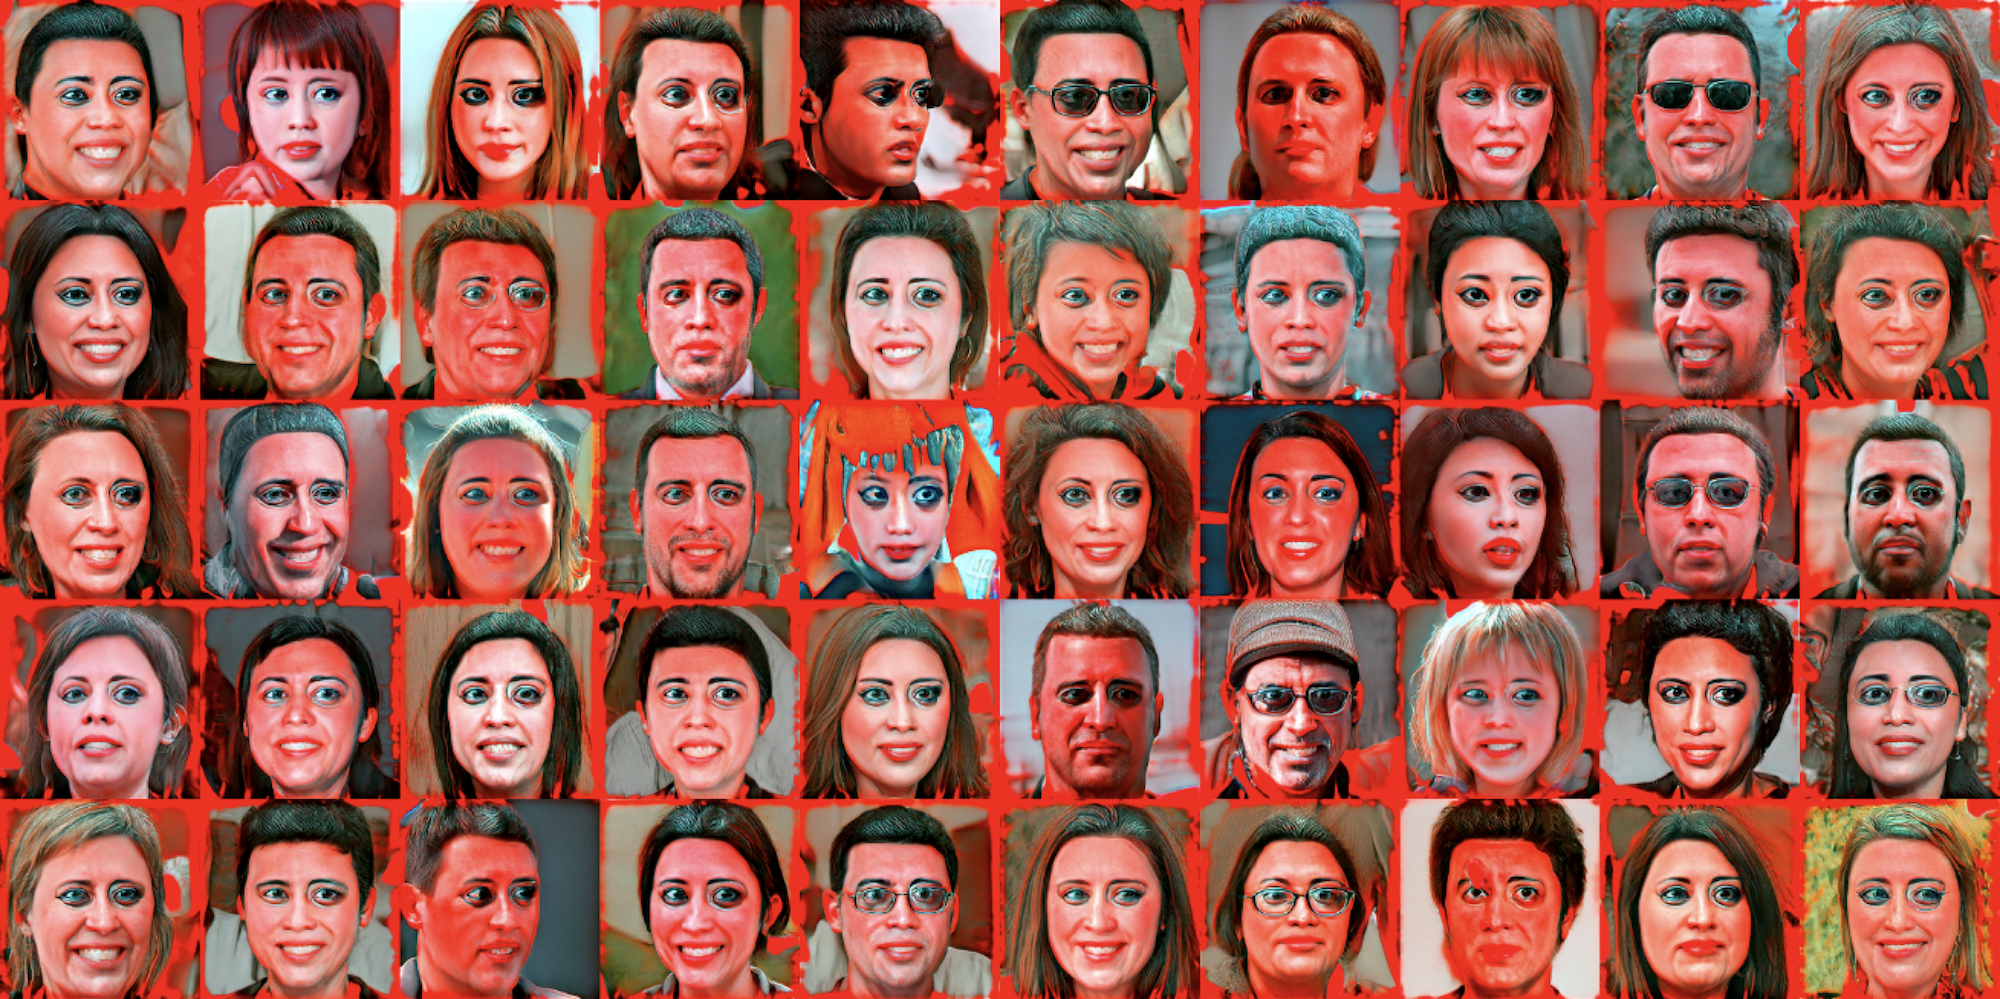
\includegraphics[width=1\textwidth]{figures/c7_impact/being-foiled.png}
    \caption{\textit{Being Foiled} (2020).}
    \label{fig:c7:being-foiled}
\end{figure}

The paper Amplifying the uncanny, which described the second set of experiments in Chapter \ref{ch:divergent}, after being published in xCoAx was cited by \cite{berns2020bridging} in their paper ‘Bridging generative deep learning and computational creativity’. 
It was in this paper that they coined the term active divergence, in an original taxonomy with four categories: latent space search, cross-domain training, early stopping and rollbacks and loss hacking. 
Where the last category, loss hacking describes the work described in Chapter \ref{ch:divergent} . 
This paper inspired the expanded survey and taxonomy of active divergence methods that I wrote in collaboration with Sebastian Berns and Simon Colton \citep{broad2021active}, detailed in the previous chapter.

The idea of freezing the weights of the discriminator and using them for fine-tuning, was used in both experiments in Chapter \ref{ch:divergent}, and was used independently in the \textit{freezing the discriminator} method \citep{mo2020freeze}. In this work, only the lower layers of the discriminator model were frozen, which was then used to aid and assist in the fine-tuning step.
Investigating the representations of the frozen discriminator network after training was performed by \citet{porres2021discriminator} in his paper, discriminator synthesis, using the gradient methods popularised in the deep dream algorithm to visualise internal feature activations of the discriminator network.

The experiments described in Chapter \ref{ch:divergent} were the first published descriptions of methods for performing divergent fine-tuning without relying on imitation-based learning. 
Subsequent approaches are detailed in \S \ref{survey:divergent}.

\section{Artworks made with network bending}
\label{c7:sec:net-bend-artworks}

A number of artworks have been made with the network bending framework, by myself, and by others. 
This section will detail them in a mostly chronological order.

\subsection{\textit{Teratome}}
\label{c7:subsubsec:teratome}

Early on in the experimental development of the network bending framework, I was hand-coding modifications to the neural network code and seeing the respective changes. 
These were simple point-wise mathematical operations, like ablation $x*0$ and inversion $x-1$ on the feature maps. 
The most significant effect of these manipulations occurred in the first few layers of the generator. 
In my initial experiments, I hard-coded these transformations into the model. Initially, I would perform this layer-wide, and later on, I was performing these to a random selection of the feature maps in a single layer. 

One of the things that struck me when examining the randomly selected manipulations of feature maps within a layer, was that in 1 in 50 or 100 images, recognisable characteristics would be preserved or altered in ways not seen in the other samples. 
For instance, eyes, and mouth, would be intact in the generated results. This exploratory stage of work is what led to the intuition that groups of features, rather than the approach of examining individual features taken by the GAN Dissection approach \citep{bau2019semantic}, would be important to allow for my semantically meaningful control and manipulation of the generated results (\S \ref{c5:sec:clustering}). 

These early experimental images (developed in 2019) were not publicly disseminated until I had published the first pre-print of the network bending paper.
I later revisited them and hand-picked some of the most striking results as a series of artworks named \textit{Teratome} \citeyearpar{broad2020teratome}  (Fig. \ref{fig:c7:teratome}). 
The name was inspired by their resemblance to teratomas, which are tumours that can contain hair, teeth and bone. 

\begin{figure}[!htbp]
    \subfloat{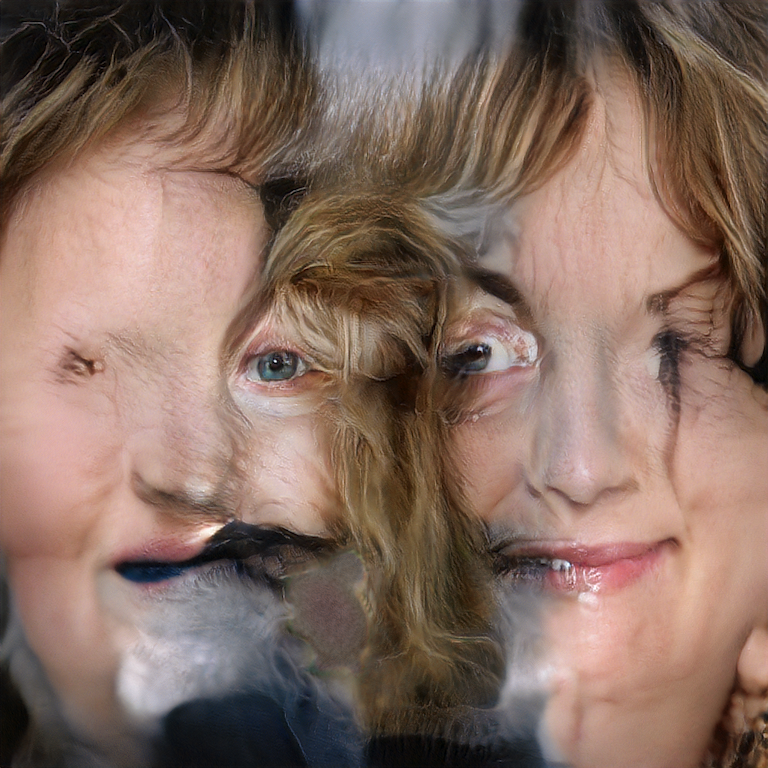
\includegraphics[width=.48\textwidth]{figures/c7_impact/teratome/1.png}}
    \hfill
    \subfloat{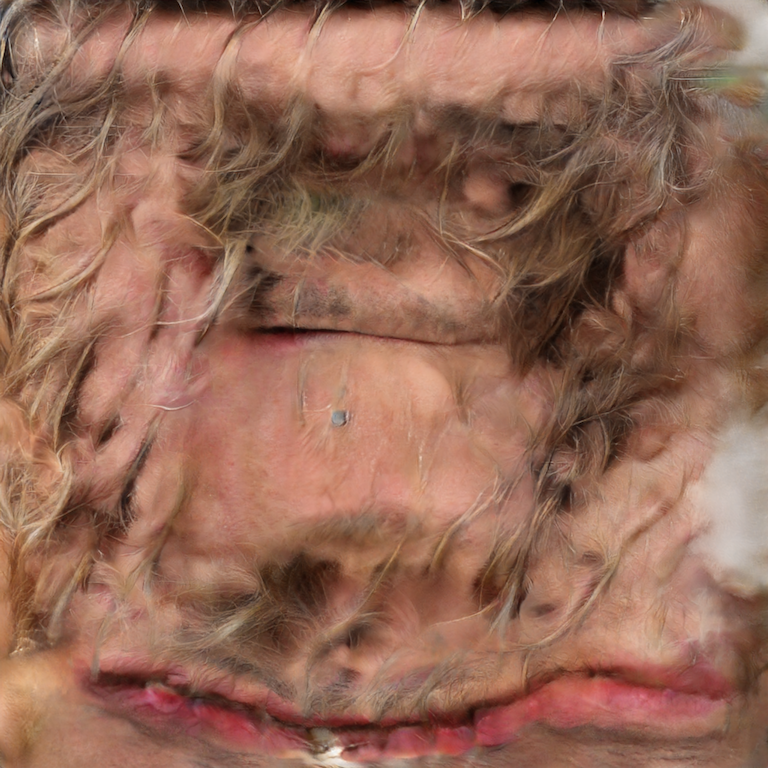
\includegraphics[width=.48\textwidth]{figures/c7_impact/teratome/2.png}}
    \hfill
    \subfloat{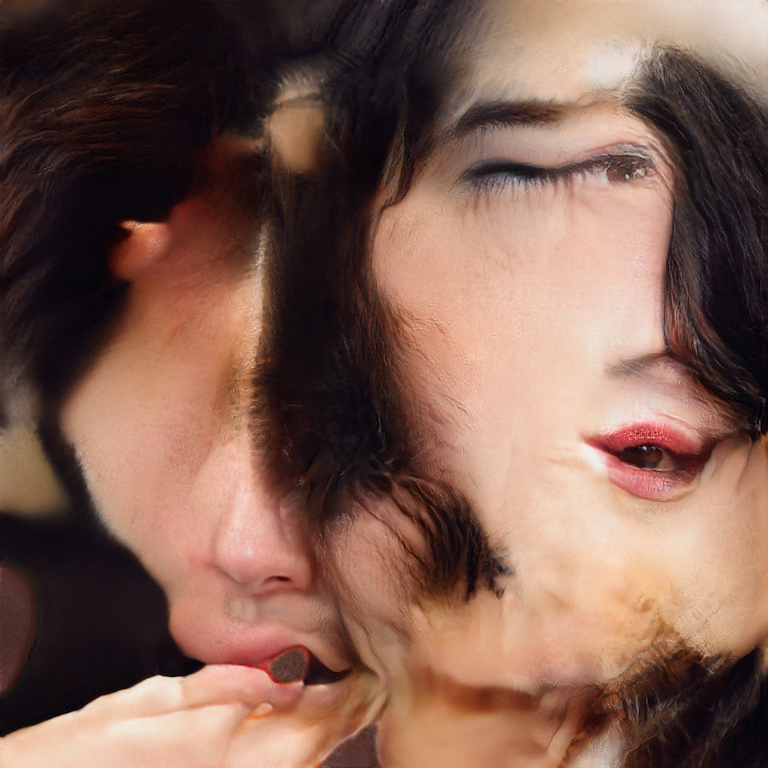
\includegraphics[width=.48\textwidth]{figures/c7_impact/teratome/3.png}}
    \hfill
    \subfloat{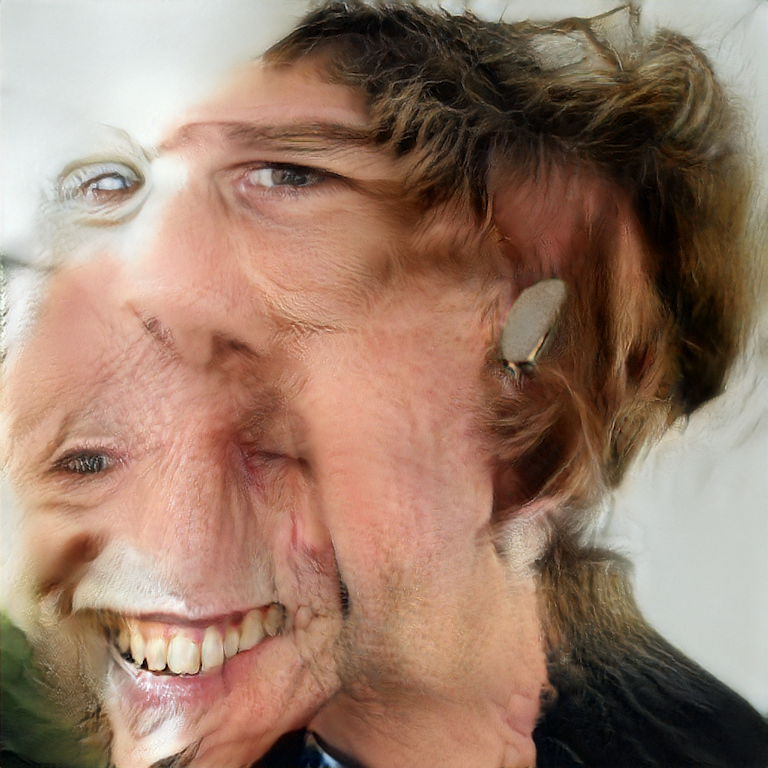
\includegraphics[width=.48\textwidth]{figures/c7_impact/teratome/4.png}}
    \caption{\textit{Teratome} (2020).}
    \label{fig:c7:teratome}
 \end{figure}


The works from the series \textit{Teratome} were one of the jurors selected works in the NeurIPS AI Art Gallery in 2020 \citep{broad2020teratome} and the HCI-Art gallery at the CHI conference in 2022 \citep{perry2022art}. 
These were later included in the subsequent book publication \textit{`The State of the (CHI)Art'} \citep{sturdee2023chiart}. 

\subsection{\textit{Disembodied gaze}}
\label{c7:subsubsec:disembodied}

Another artwork that was made during the development of the network bending framework was the work \textit{Disembodied gaze}. 
This was made shortly after I completed the work on the clustering algorithm and investigated the results. 
One of the clusters from the algorithm that had the clearest effect was the cluster in layer 5 that determined the generation of eyes (\S \ref{c5:sec:clustering}). 
When the cluster is ablated, the eyes disappear and the model fills in the gaps with skin  (Fig. \ref{fig:c7:eyes-no-eyes}). 
This alone was quite a surprising result. But when all the features but the eyes are ablated, things get a lot more surprising. 

\begin{figure}[!htbp]
    \subfloat[]{\label{subfig:eyes}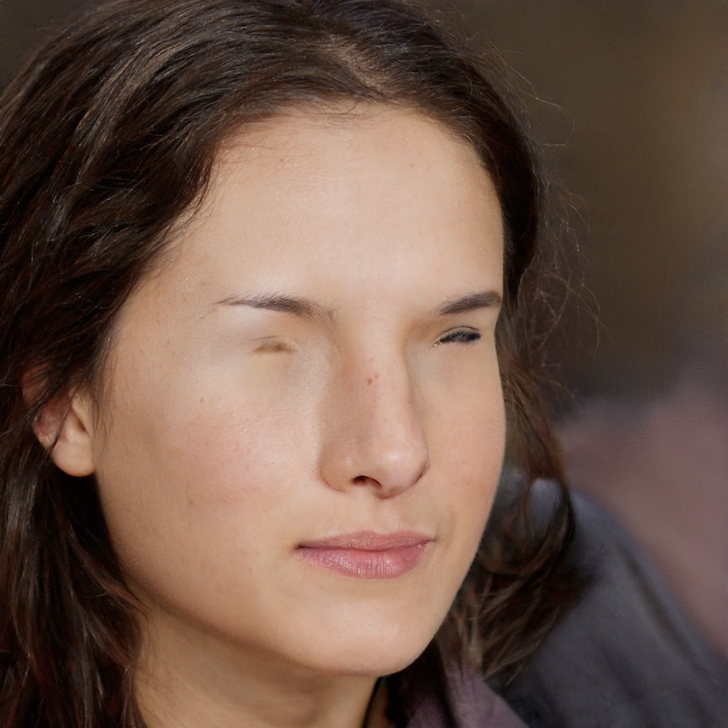
\includegraphics[width=.48\textwidth]{figures/c7_impact/eyes-off.png}}
    \hfill
    \subfloat[]{\label{subfig:no-eyes}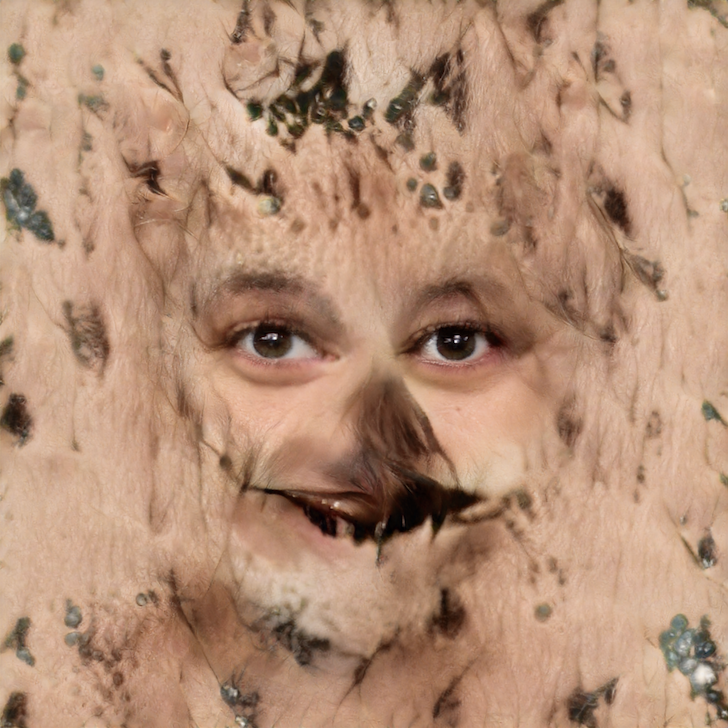
\includegraphics[width=.48\textwidth]{figures/c7_impact/eyes-on-face-off.png}}
    \hfill
    \caption[Network bending eye cluster comparison]{(a) Image generated using network bending with cluster controlling the generation of eyes ablated. (b) Image generated with network bending where all convolutional features apart from those that generate eyes are ablated.}
    \label{fig:c7:eyes-no-eyes}
 \end{figure}

I was struck by the bizarre textural regions that were filled in the background, and the ghostly smile that emerges from this absence. 
I experimented with making a latent interpolation video with this model. GAN latent space interpolations were very popular back in 2016-2020, and I personally was not that keen on them.
I found the constant morphing of them quite nauseating and I felt like they were quite a cheap trick to do with any newly trained GAN model, relying on a tendency in AI art that Zylinska describes as `dazzling viewers with the mathematical sublime of big data sets, rapid image flows and an intermittent flicker of light, sound and movement' that ends up `ends up serving as a PR [public relations] campaign for corporate interests' \citeyearpar{zylinska2020ai}. 
However, with the network bending intervention, I did not get the nauseating effect from the constant shape-shifting in the same way. 
Though the identities were changing, so many of the recognisable characteristics were gone, leaving only the eyes as a fixed point in the video, contrasted with the stochastic nature of the constantly changing textural background. 

After making an initial video at the standard square aspect ratio (1024x1024), ubiquitous for latent space interpolation videos at the time, I set about making a work that was bigger and at a more cinematic aspect ratio. 
I developed a new network bending transformation layer that mirrored and extended the width of the activation maps by padding the sides of them with zeros.\footnote{
    I did not make this transformation layer publicly available as invalid parameters could quickly lead to the software crashing due to a segmentation fault or GPU memory error.
}
As all of these regions that were bordering the edges of the image were already ablated in the network, the effect of this padding appears seamless in the generated result. 

\begin{figure}[!htb]
    \centering
    \captionsetup{justification=centering}
    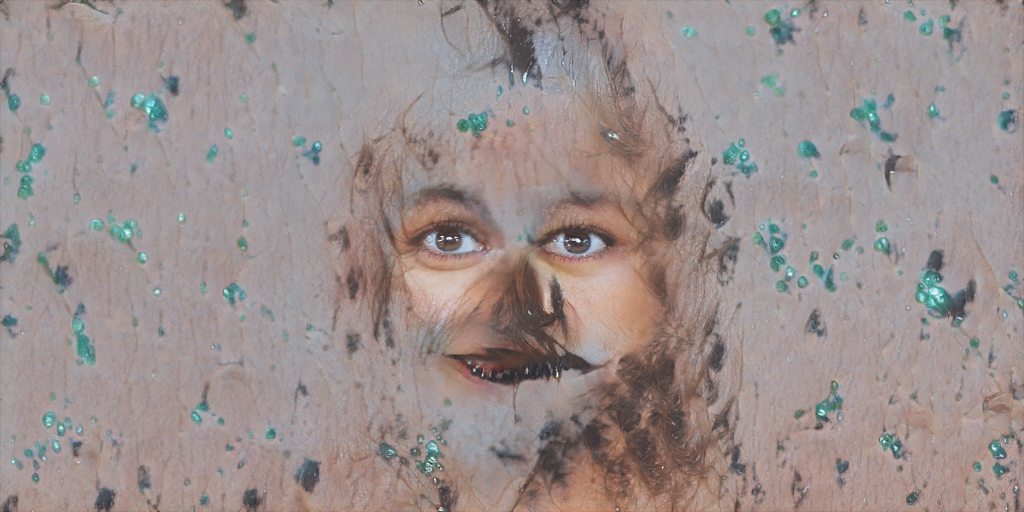
\includegraphics[width=1\textwidth]{figures/c7_impact/disembodied_gaze.png}
    \caption{Still from \textit{Disembodied Gaze} (2020).}
    \label{fig:c7:disembodied-gaze-wide}
\end{figure}

After some cropping and formatting of the video into a commonly used aspect ratio, and creating a seamlessly looping video 13 minutes in length, I created the video work \textit{Disembodied gaze} \citep{broad2020disembodied}. 
This work was never exhibited as such, but I revisit it a lot in artist talks as it is a good illustration of what is possible with network bending, and is a good demonstration of something that is unique to the approach, and would be near impossible to make any other way. 
The padding layer was also something I used later on in the \textit{Fragments of Self} work detailed in \S \ref{c7:subsubsec:fragments}.

\subsection{Single and EP Artworks for \textit{0171}}
\label{c7:subsubsec:0171}

In the spring of 2020, I was approached by musicians from the band 0171, who were releasing a series of singles, followed by an EP that autumn. 
They were keen to use images of themselves, and have them manipulated using some of the techniques that I had been developing in this PhD.
As I was using StyleGAN2, there was already existing code online that performed projection of photographs of people into the GAN latent space \citep{abdal2019image2stylegan}.
This meant that I could take portrait photographs of the two band members and project them into StyleGAN2 latent space, before then manipulating the models while generating these latent codes to make artwork for the commission. 

They provided me with one of their press shots  (Fig. \ref{fig:c7:0171-press-shot})  that was to be used for their forthcoming marketing campaign for the new singles and EP. 
I cropped the respective faces of the two band members, and projected them into StyleGAN2 latent space, using the gradient method \citep{abdal2019image2stylegan}  (Fig. \ref{fig:c7:0171-crop-embed}).

\begin{figure}[!htb]
    \centering
    \captionsetup{justification=centering}
    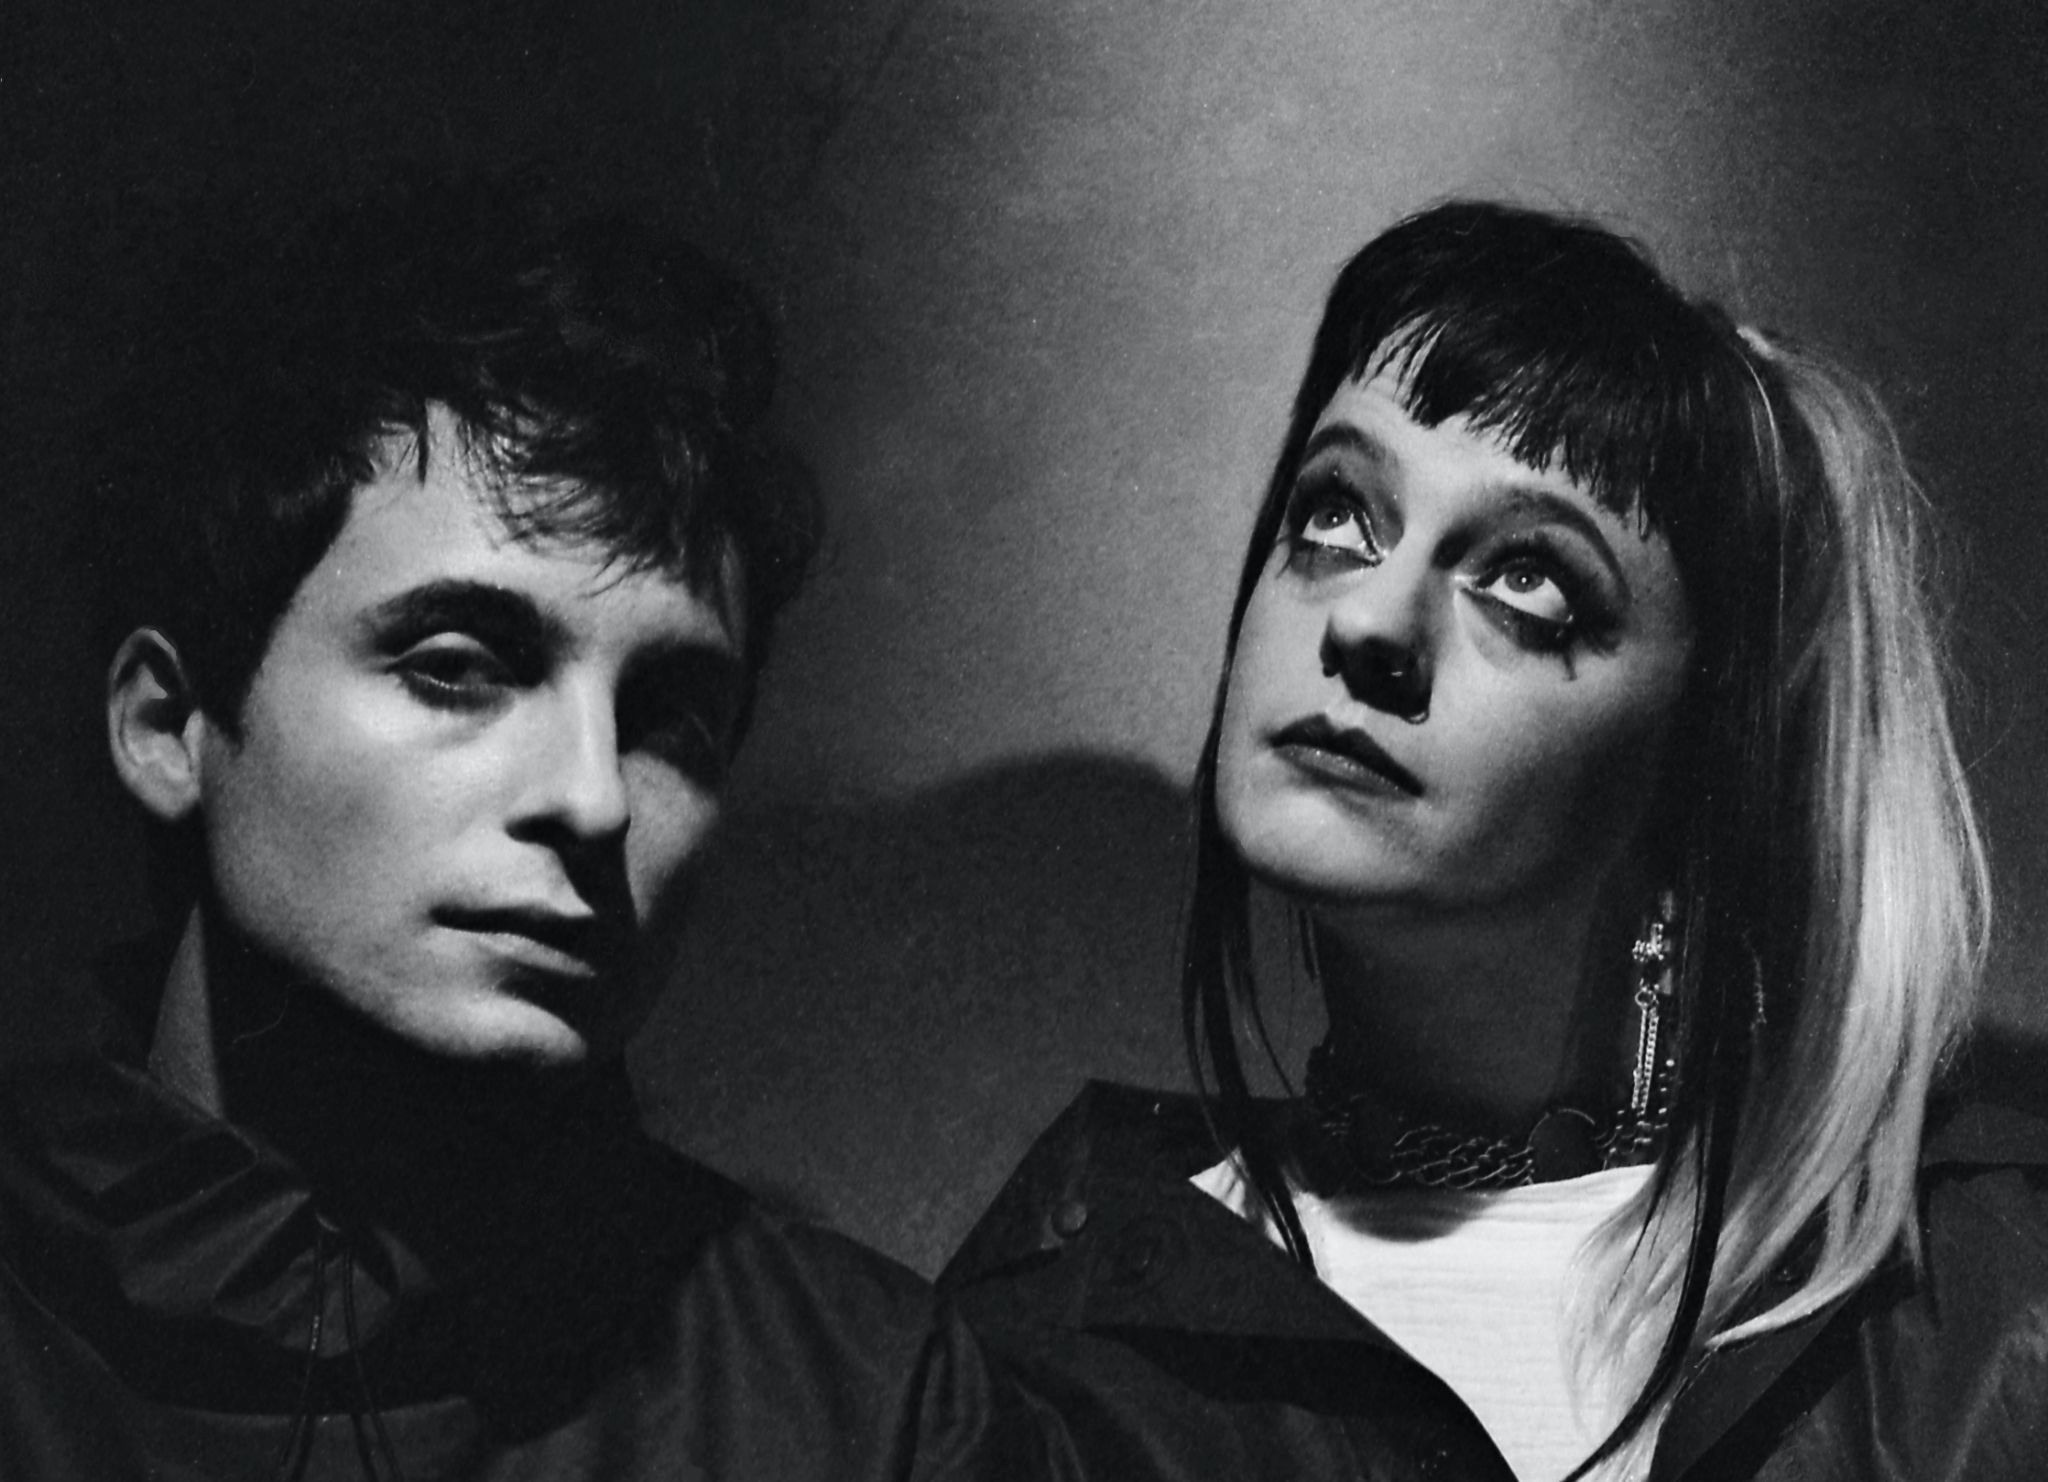
\includegraphics[width=1\textwidth]{figures/c7_impact/0171/press/0171-press-shot.png}
    \caption{0171 Press shot. Image courtesy of Georgie Hoare and Joe Bedell-Brill.}
    \label{fig:c7:0171-press-shot}
\end{figure}

\begin{figure}[!htbp]
    \subfloat[]{\label{subfig:joe-cropped}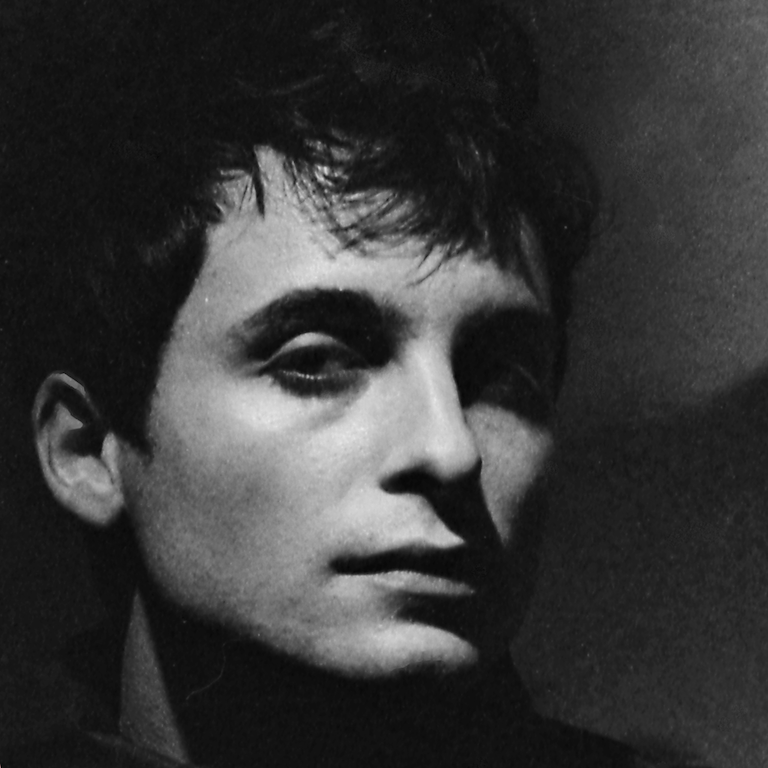
\includegraphics[width=.24\textwidth]{figures/c7_impact/0171/press/joe-cropped-press.png}}
    \hfill
    \subfloat[]{\label{subfig:joe-latent}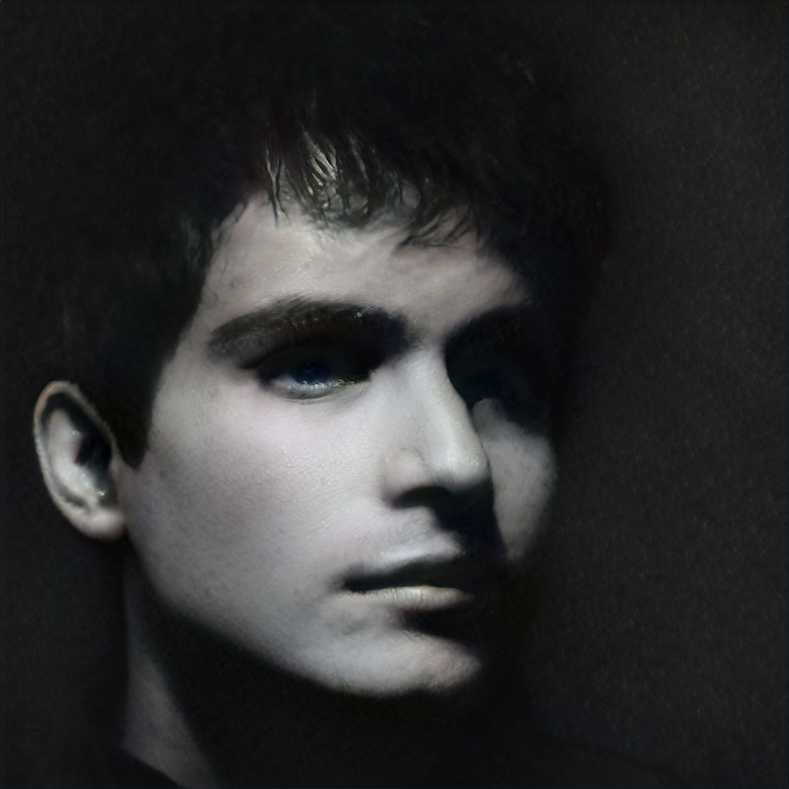
\includegraphics[width=.24\textwidth]{figures/c7_impact/0171/press/joe-cropped-style.png}}
    \hfill
    \subfloat[]{\label{subfig:georgie-cropped}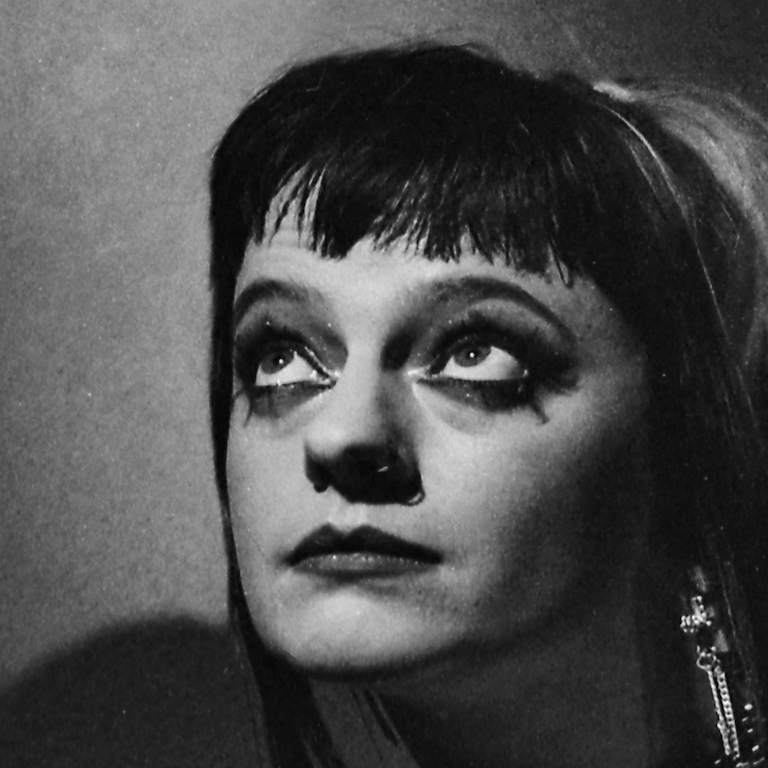
\includegraphics[width=.24\textwidth]{figures/c7_impact/0171/press/georgie-cropped-press.png}}
    \hfill
    \subfloat[]{\label{subfig:georgie-latent}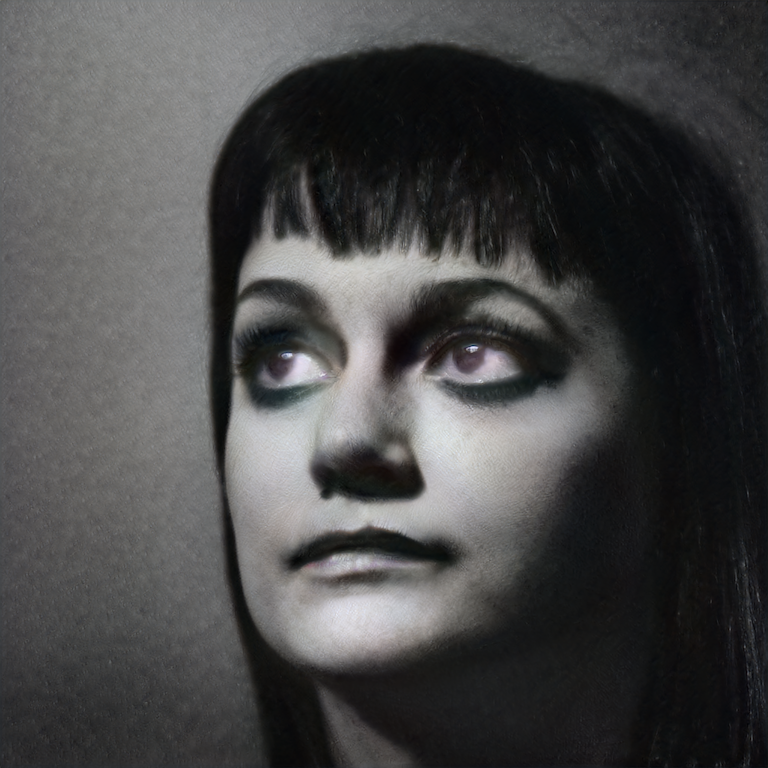
\includegraphics[width=.24\textwidth]{figures/c7_impact/0171/press/georgie-cropped-style.png}}
    \caption[0171 headshots cropped and projected into StyleGAN latent space]{Images of the individual band members cropped from the press shot (a,c) and their respective StyleGAN2 projections (b,d). }
    \label{fig:c7:0171-crop-embed}
 \end{figure}

I took an exploratory approach to find combinations of stochastic and layer-wide transformations to the models, using this as an exercise to understand how transformations could be combined to produce more divergent and original images. 
I would keep the latent the same, alternating between the latent codes for the two respective band members, testing out different configurations of transformation parameters. 
I would generate 20 images using one set, and there would always be variation in the images because of the stochastic layer transformations used. 
There would be more significant variation if these were used in the earlier layers of the GAN, or if the percentage of random features distorted with a transformation was increased.

I would experiment intuitively with different configurations of transformations. 
If the set of results did not have much interesting variation I would boost the random threshold for features applied, and if it had too much I would tone these down. 
If one configuration produced a particularly fruitful set of results, I would generate more using the same parameters -- i.e. 100 or 1000. 
After experimenting like this for several days I selected my favourite samples and shared those with the band.

\begin{figure}[!htbp]
    \subfloat[]{\label{subfig:joe-h-1}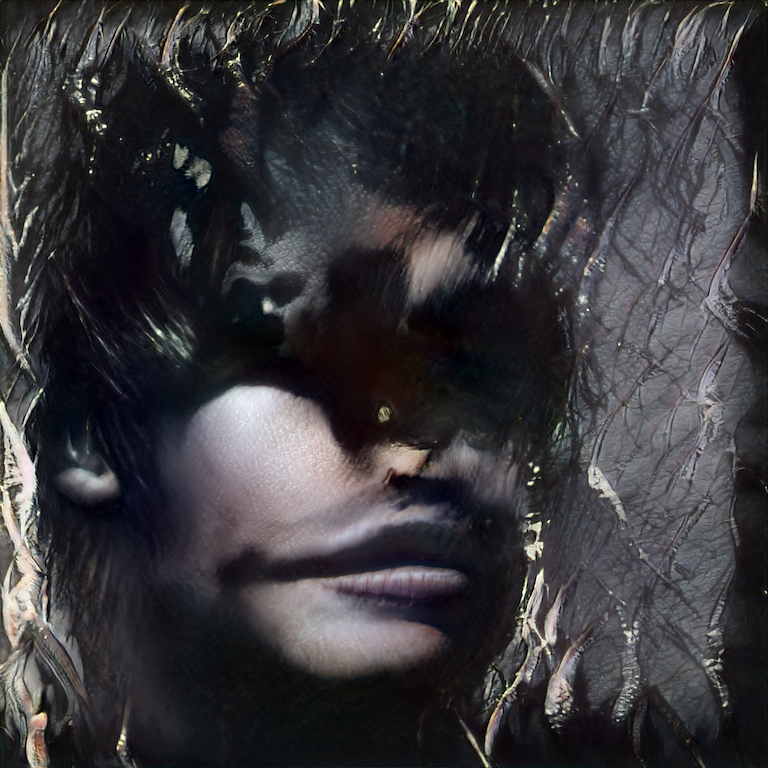
\includegraphics[width=.32\textwidth]{figures/c7_impact/0171/haunted/joe-1.png}}
    \hfill
    \subfloat[]{\label{subfig:joe-h-2}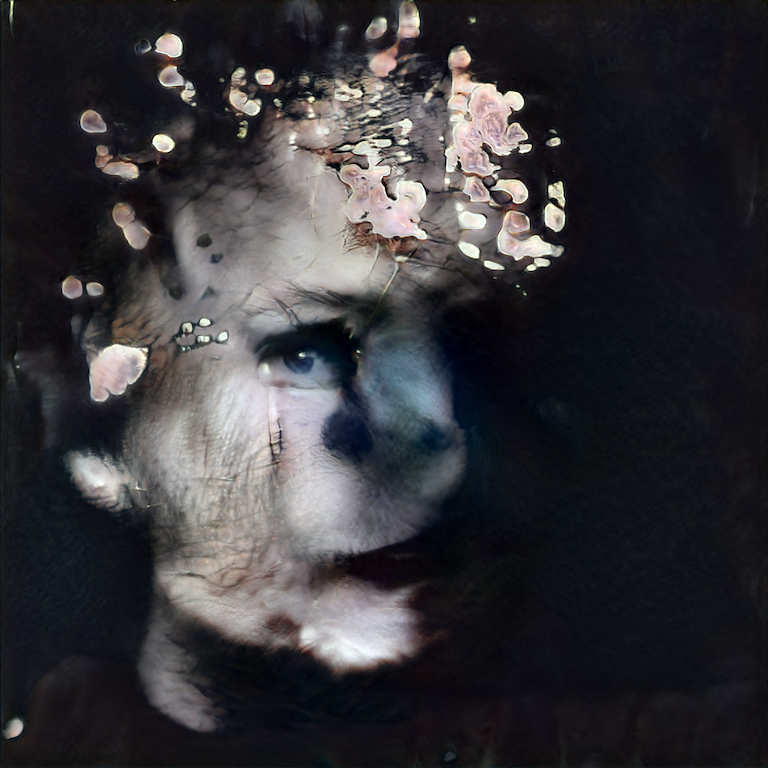
\includegraphics[width=.32\textwidth]{figures/c7_impact/0171/haunted/joe-2.png}}
    \hfill
    \subfloat[]{\label{subfig:joe-h-3}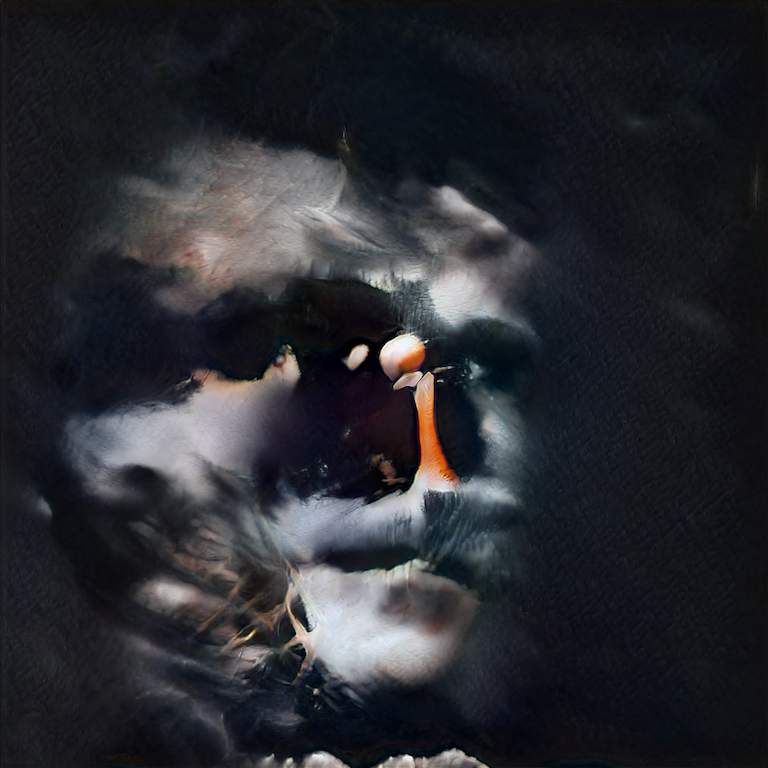
\includegraphics[width=.32\textwidth]{figures/c7_impact/0171/haunted/joe-3.png}}
    \hfill
    \subfloat[]{\label{subfig:georgie-h-1}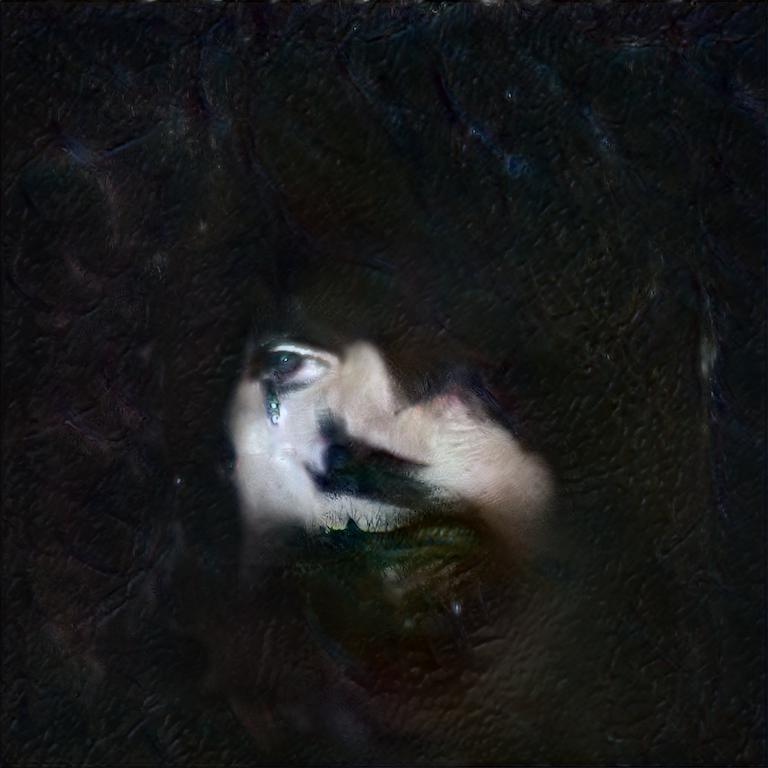
\includegraphics[width=.32\textwidth]{figures/c7_impact/0171/haunted/georgie-1.png}}
    \hfill
    \subfloat[]{\label{subfig:georgie-h-2}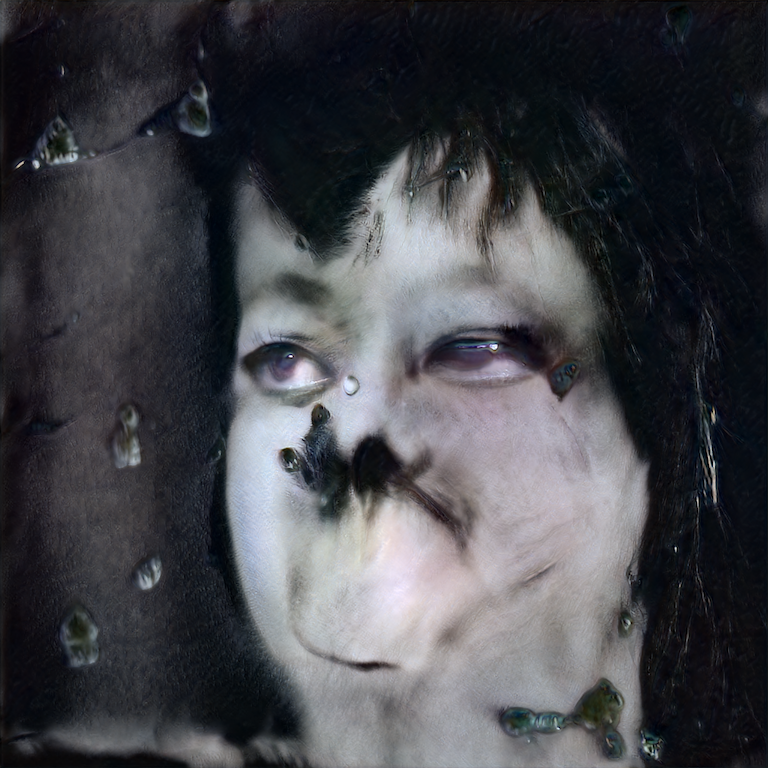
\includegraphics[width=.32\textwidth]{figures/c7_impact/0171/haunted/georgie-2.png}}
    \hfill
    \subfloat[]{\label{subfig:georgi-h-3}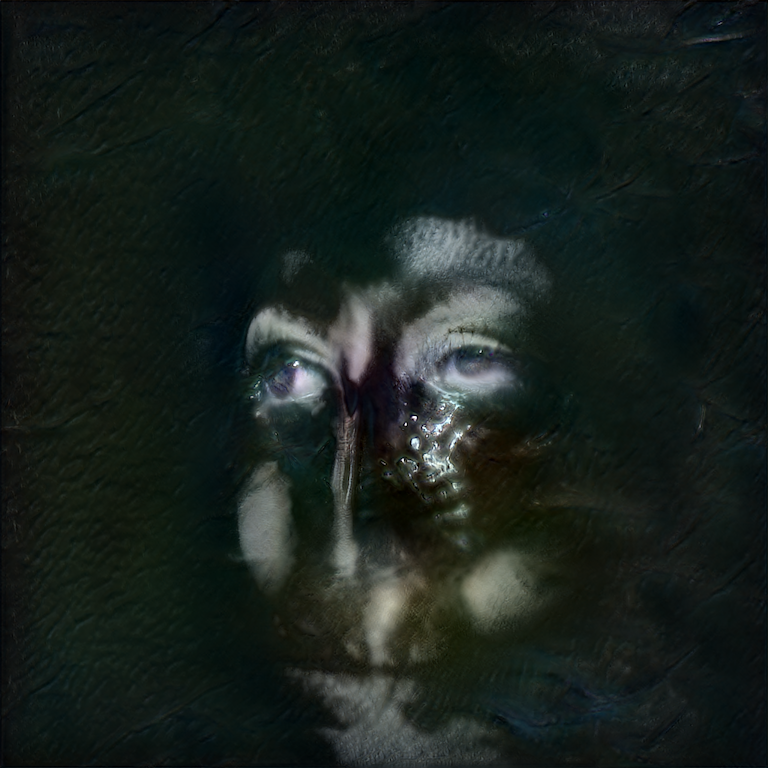
\includegraphics[width=.32\textwidth]{figures/c7_impact/0171/haunted/georgie-3.png}}
    \hfill
    \caption[Network bending applied to 0171 headshots]{(a-c) images generated using network bending techniques applied to the latent \ref{subfig:joe-latent}, (d-f) images generated using network bending techniques applied to the latent \ref{subfig:georgie-latent}.}
    \label{fig:c7:0171-haunted}
 \end{figure}

I shared these original works with the band, and while they were very impressed with the result, they were not quite in line with the desired aesthetic for a synth-pop band. 
The original images were sourced from a dark, black-and-white film photograph, which had been deliberately distorted with scratches and other physical interventions made to the film. 
As the latent codes were conditioned on this image, the dark, gothic look was persistent in the results and accentuated by the facial distortions present  (Fig. \ref{fig:c7:0171-haunted}). 
I advised them that if they wanted something more colourful and pop-friendly, then using a different more colourful image of themselves as the starting point would work better.
They provided me with headshots taken in front of a colourful painting, which we then used for the project. 

I began repeating the process described earlier with the previous latent codes of the band members. 
Trying out the same transformation parameters that produced interesting results with the previous latent codes, and adapting them to work better with the new ones. 
Not all transform configuration settings that worked with the previous latent codes worked well with these, without some tweaking. 
Showing that there was a clear contingency between how well different latent codes and transform parameter configurations would work well together.
In addition, based on feedback from the band members that the distorted but recognisable faces were also not aligned with the appearance the band were trying to give off, I increased the level of distortion so that the generated images appeared more abstract than with the initial attempt  (Fig. \ref{fig:c7:0171-haunted}). 
This time, the band members themselves were more involved in the process. I would experiment with transformation parameters, select some of my personal favourites, and show these to the band who would tell me what they liked and disliked and that would inform further experimentation. 
We ended up with 10 pictures, 5 for each band member, and they selected their favourite of these for the 4 EP and single releases  (Fig. \ref{fig:c7:0171-EP}). 

\begin{figure}[!htbp]
    \subfloat[]{\label{subfig:ep1}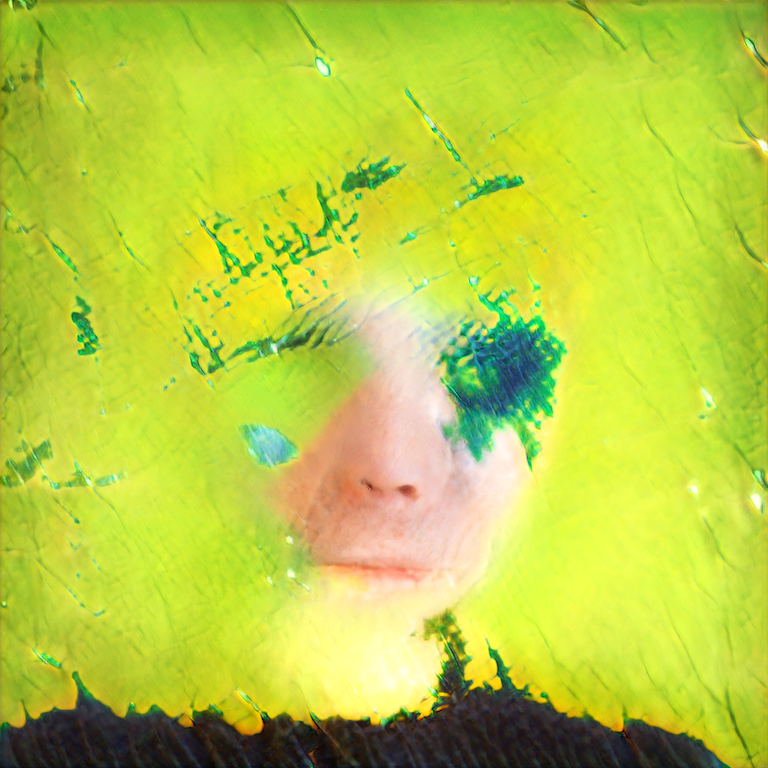
\includegraphics[width=.48\textwidth]{figures/c7_impact/0171/ep/automatic.png}}
    \hfill
    \subfloat[]{\label{subfig:ep2}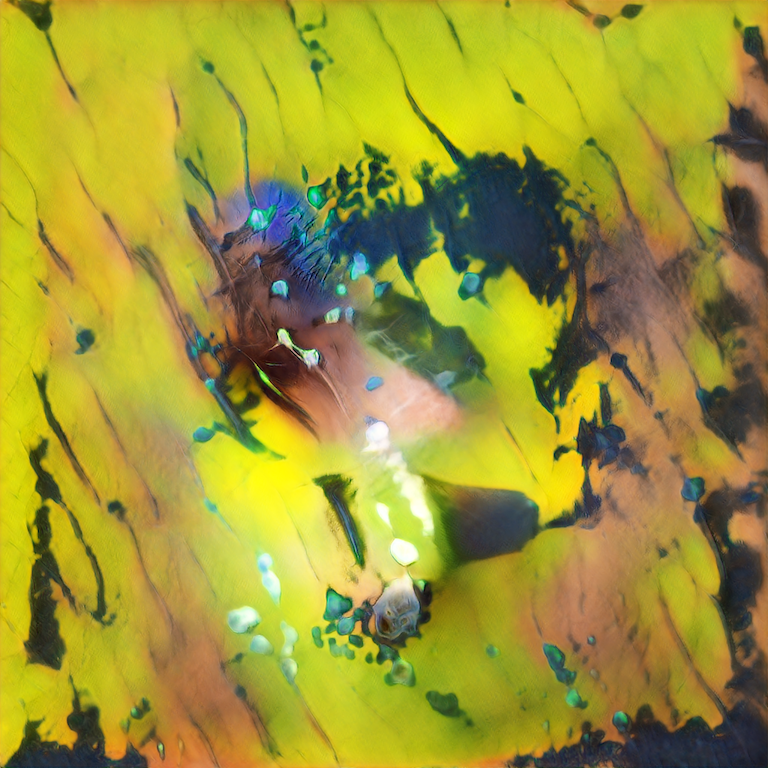
\includegraphics[width=.48\textwidth]{figures/c7_impact/0171/ep/follow.png}}
    \hfill
    \subfloat[]{\label{subfig:ep3}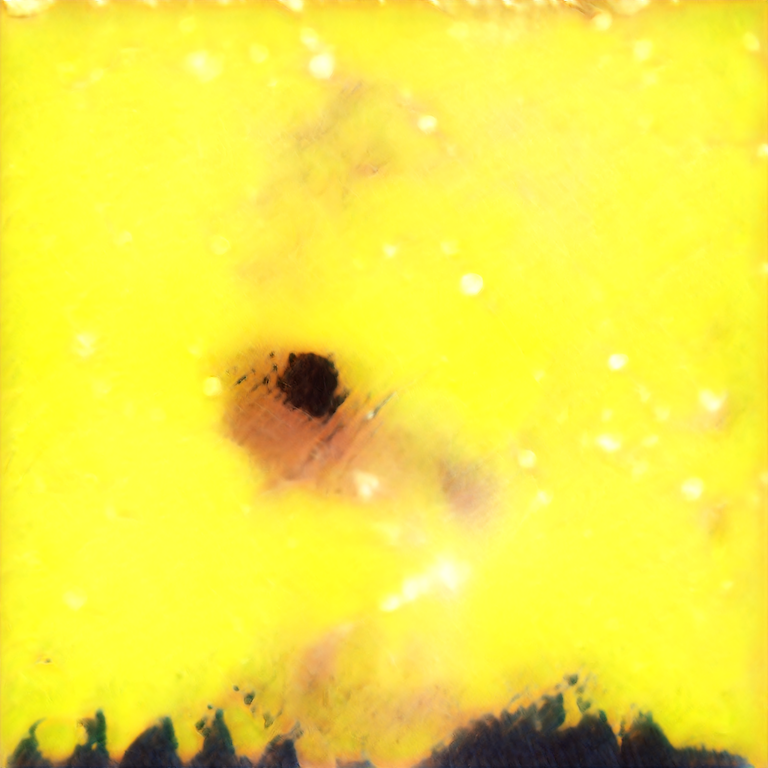
\includegraphics[width=.48\textwidth]{figures/c7_impact/0171/ep/photograph.png}}
    \hfill
    \subfloat[]{\label{subfig:dp4}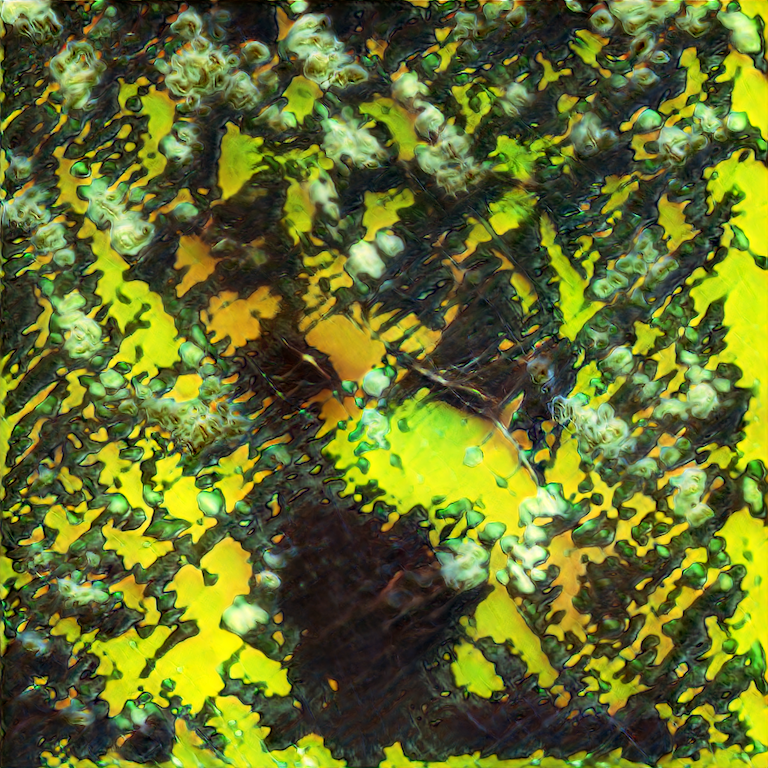
\includegraphics[width=.48\textwidth]{figures/c7_impact/0171/ep/change-nothing.png}}
    \caption[0171 EP artworks]{EP and single artworks created for the band 0171. (a) Artwork for single \textit{Automatic}. (b) Artwork for the single \textit{Follow}. (c) Artwork for the single \textit{Photograph}. (d) Artwork for the EP (extended play) compilation \textit{Change Nothing}.}
    \label{fig:c7:0171-EP}
 \end{figure}

Working on this series of artworks as the network bending framework was in development was fortunate in its timing as it served as a useful case study early on in the development of this framework in a real-world application, and later detailed in the original EvoMUSART paper \citep{broad2021network} 
The single and EP artworks are available to see on all good music streaming services.
The earlier images (in Figure \ref{fig:c7:0171-haunted}) were later used (with permission from the band) to produce the NFT artworks Haunted Variations \citep{broad2021haunted1,broad2021haunted2}. 

\subsection{\textit{Fragments of self}}
\label{c7:subsubsec:fragments}

After producing some striking visuals with the transformations of the band members, I would have been remiss if I were not to have performed the same transformations myself. 
I took a self-portrait photograph of myself from a holiday in Croatia and projected that into StyleGAN2 latent space. 


\begin{figure}[!htbp]
    \subfloat[]{\label{subfig:selfie-og}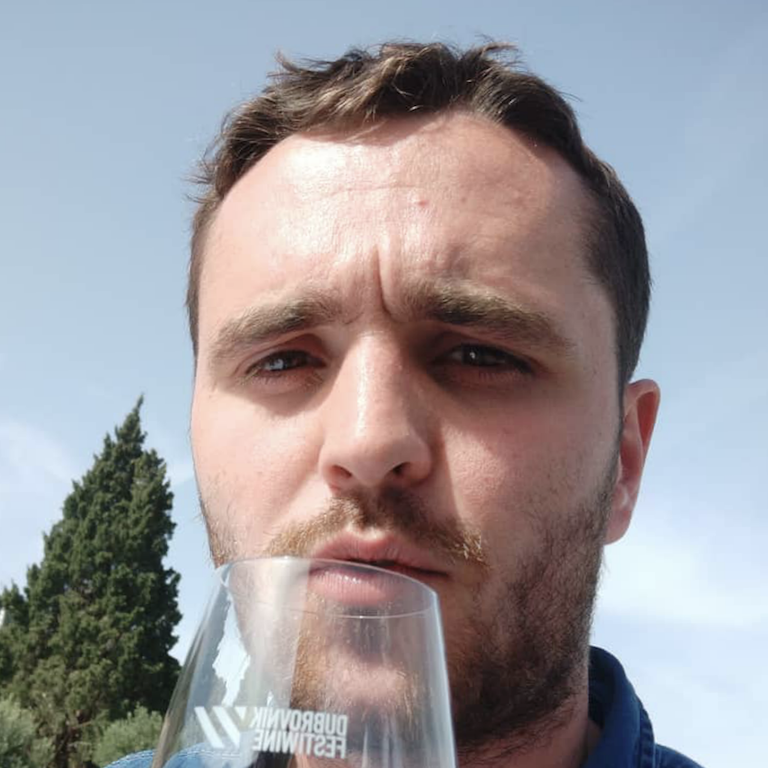
\includegraphics[width=.48\textwidth]{figures/c7_impact/selfie/og.png}}
    \hfill
    \subfloat[]{\label{subfig:selfie-latent}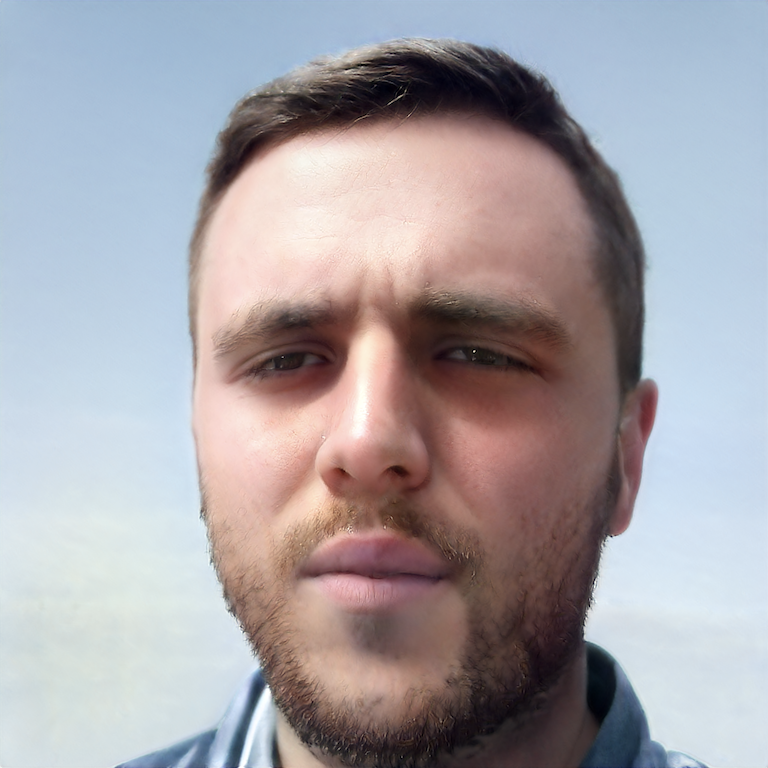
\includegraphics[width=.48\textwidth]{figures/c7_impact/selfie/latent.png}}
    \hfill
    \caption[Selfie and latent projected into StyleGAN2 latent space comparison]{(a) Original selfie photograph of myself. (b) Closest match to (a) in StyleGAN2 latent space.}
    \label{fig:c7:selfie}
 \end{figure}

I took some of the random transformation configurations that were used for the final 0171 EP artworks and tried them on myself, but these were rendering images that were largely unrecognisable from myself. 
Therefore, I reduced the number of convolutional filters that were being affected by the random layer filters and reduced some of the other parameters such that the results were more clearly recognisable  (Fig. \ref{fig:c7:selfie-series}).


\begin{figure}[!htb]
    \centering
    \captionsetup{justification=centering}
    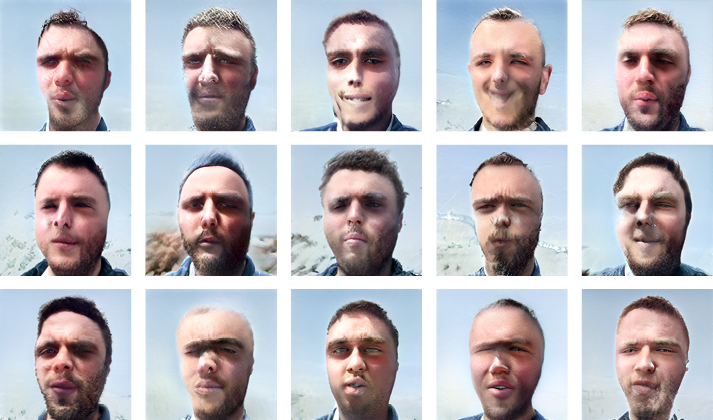
\includegraphics[width=1\textwidth]{figures/c7_impact/selfie/selfie-series.png}
    \caption[Samples of selfies distorted with random network bending parameters]{ Samples of selfies distorted with random network bending parameters based on the latent \ref{subfig:selfie-latent}.}
    \label{fig:c7:selfie-series}
\end{figure}


None of these images, by themselves, were particularly close to my own recognition, as the level of distortion was still quite high.
As I was navigating through them in the image viewer, I noticed that if I held these keys and scrolled quickly through the images, as if they were in motion, the resemblance to myself was much stronger. 
I ended up stitching together 1000 of these randomly generated images into a looping video approximately 10 seconds long and making a short video piece that was shared on social media. 
Like the work \textit{disembodied gaze} (\S \ref{c7:subsubsec:disembodied}), this was not exhibited anywhere but is something I share regularly in artist talks as it is an instructive illustration of the possibilities offered by the network bending framework.
It was not until I was invited to participate in the upcoming exhibition for the digital art gallery platform Feral File (created by Casey Raes), that this line of enquiry had any major impact. 

I was unsure of what I was going to exhibit in this show, but I was given the curator notes from Luba Elliot several months in advance for the exhibition opening, where she had decided on the title \textit{Reflections in the water}:

\begin{quote}
`Working with AI art sometimes feels like gazing into a pond of water — we are not sure what we will get as a reflection. [...] Looking into a still pond, we see a clear, gently blurred version of ourselves staring back at us, while turbulent waters return mere rippled echoes of our shape. These changing reflections of ourselves are similar to images generated from data, which can be hyper-realistic depictions of the original, or images that are surreal and barely recognizable, as flaws and errors creep in. [...]

GAN technologies have improved much over the years [...] present[ing] a surprising challenge to AI art practitioners—what to do now that perfect realism is within reach? [... W]orking with AI has the potential to change too, as the technology becomes more predictable and controllable, rendering blurry reflections, distorted forms and uncertain outcomes a thing of the past.' \citep{elliot2021reflections}.
\end{quote}

I was inspired by some of the passages in these exhibition notes and wanted to make an artwork that best fit with the theme. 
The description of seeing a distorted representation of ourselves reflected in the results of AI-generated images rang particularly true, reflecting on the experiment with the selfies that I detailed here.

Using headshot photographs of myself, I began projecting them into the StyleGAN2 latent space and experimenting with network bending on them. 
In the latent for one of these headshots, the background became oversaturated off-white and was quite uniform. 
When ablation was applied to this, the face disappeared into the uniform background. 
Applying random ablation to filters in layer 5 of StyleGAN2 gave a strong resemblance to gazing at my own reflection in distorted waters.
I set about creating an animated sequence that was as closely aligned to that visual metaphor as I could.

Sequencing frames where transformations are applied at random between each frame, as I had done with the images from Figure \ref{fig:c7:selfie-series} made for very chaotic viewing, which did not really correspond to the imagery of looking at a reflection in the water.
Therefore, I set about creating a more coherent temporal way of interpolating between random selections of features in a layer to manipulate. 
I opted to use Perlin noise, where I could render a tensor of 3 dimensions, that would give a smooth transition between states in the tensor.
I used one of the dimensions of the tensor to represent time, and the other dimension was used to map to each filter in a convolutional layer in the StyleGAN2 network.
I would then use a threshold to determine whether a convolutional filter would be ablated or not in the GAN model.
This threshold could be adjusted manually to get the right configuration of filters being ablated at any one time in order to get the desired visual effect, where a small fragment of my face could only ever be seen in a single frame, but when watched in motion, my overall resemblance would be seen in constructed in the viewers mind. 

The final work was titled \textit{Fragments of Self} \citeyearpar{broad2021fragments}  (Fig. \ref{fig:c7:fragments}). 
During the creation of this work, I was  drawn to these images of fragmented versions of myself. 
On reflection, I can see that I was making this work during my recovery from Long-COVID, where during this period of chronic illness, I never felt like a whole person.\footnote{
    I was one of the unfortunate people who contracted COVID-19 in the first wave in the UK, just before the March lockdown of 2020. 
    Shortly after recovering, I became seriously ill with Post-COVID Syndrome, aka Long-COVID.
    For close to twelve months, an ever-changing set of physical and cognitive impairments made it nearly impossible for me to work on my PhD, and I did not fully recover until two years after I first became ill.
} 
This illness was a constant barrage of changing ailments and symptoms, which left me with the feeling of being a fragment of my former self for a very long time.

\begin{figure}[!htbp]
    \centering
    \subfloat{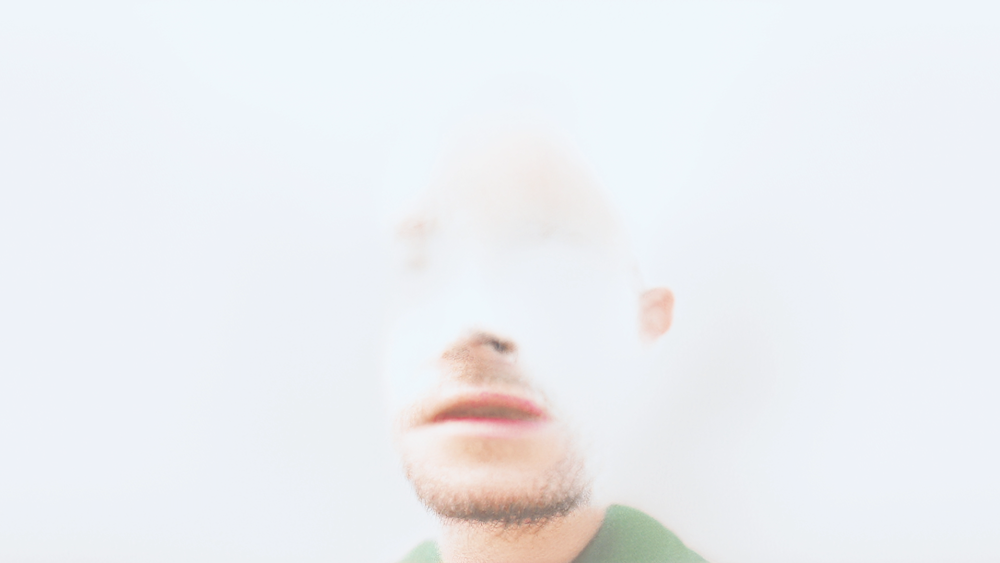
\includegraphics[width=.9\textwidth]{figures/c7_impact/fragments/2.png}}
    \hfill
    \subfloat{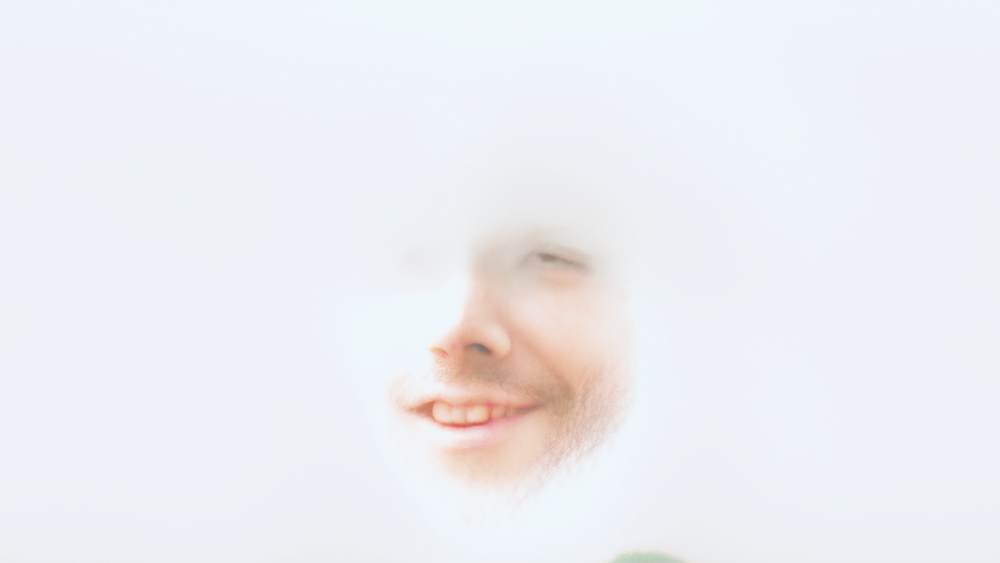
\includegraphics[width=.9\textwidth]{figures/c7_impact/fragments/3.png}}
    \hfill
    \subfloat{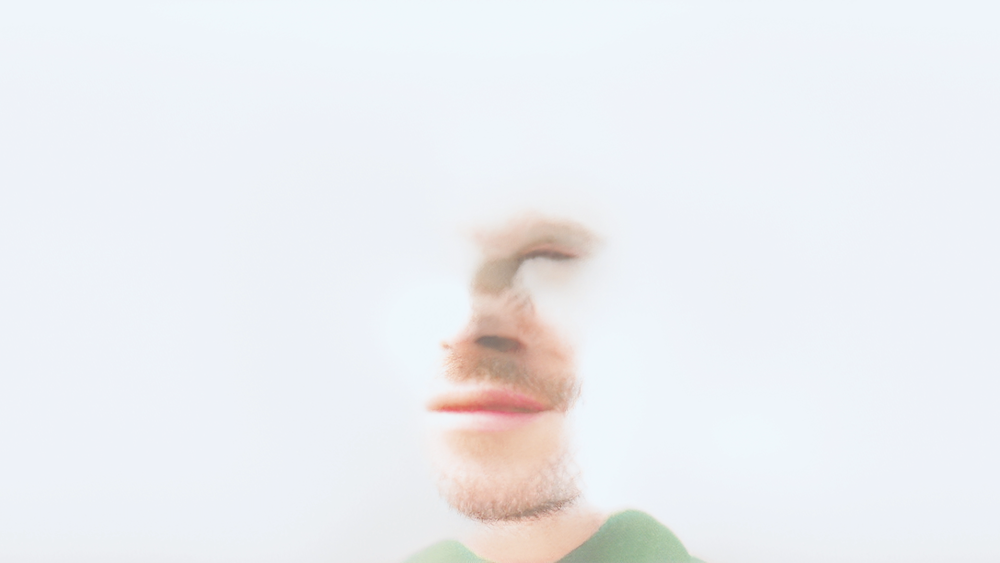
\includegraphics[width=0.9\textwidth]{figures/c7_impact/fragments/4.png}}
    \caption[Stills from \textit{Fragments of Self}]{Stills from \textit{Fragments of Self} (2021).}
    \label{fig:c7:fragments}
 \end{figure}

\subsection{Jen Sykes' \textit{Field of View} and \textit{The Offing}}

Jennifer Sykes is an artist, designer and lecturer based between Glasgow, Scotland and London, England, where she teaches at the UAL Creative Computing Institute.
She has used network bending in the production of several artworks. Building on a prior work, \textit{Places You’ve Never Been} \citep{sykes2018places}, which used an archive of digitised film slides, captured from her family's migration from Canada to England, which was later used that to train a generative model. 

In \textit{Fields of View}, uses the clustering algorithm of network bending to `change our interpretation to isolate “semantic groupings" that include only the sky or only the mountains of a specific narrative?' \citep{sykes2021fields}. 
Exploring the personal archive of family images of migration, network bending is used to produce a selective generation of aspects of those archival images. 
Sykes likens this process to `historic in-camera editing techniques of cameraless film-making' \citep{sykes2021fields} as the manipulation is happening to the features present within a dataset, with no new footage being needed.

In \textit{The Offing}  (Fig. \ref{fig:c7:offing}), the same dataset and network bending transformations to manipulate landscape images. 
Here, clusters have been isolated that relate to the sky and the land, and these images are rotated in an animated sequence. 
The work produces a `narrative stitched together through layers of the horizon; where land meets the sea'  \cite{sykes2022offing}, which is colloquially referred to as the offing. 

\begin{figure}[!htbp]
    \subfloat{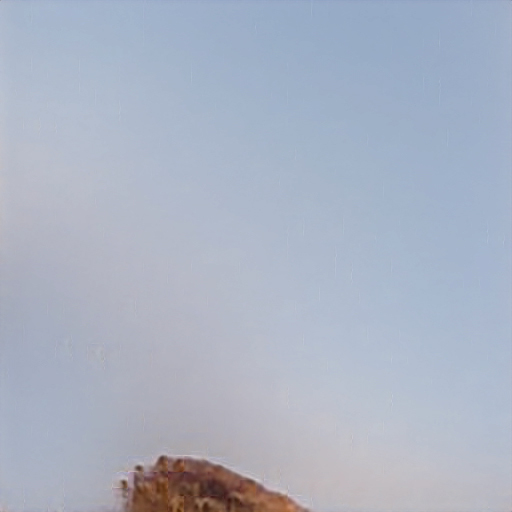
\includegraphics[width=.33\textwidth]{figures/c7_impact/other-artworks/offing/4.jpg}}
    \subfloat{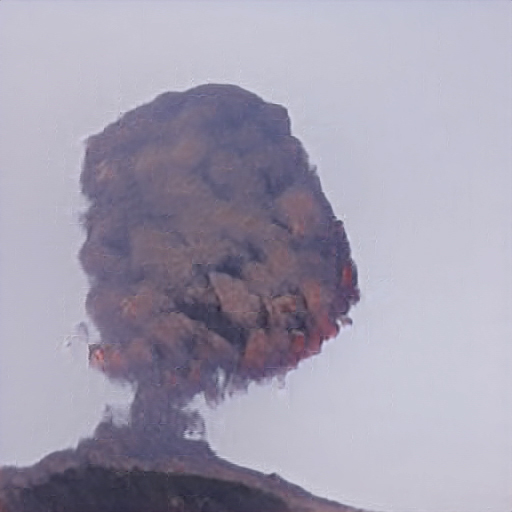
\includegraphics[width=.33\textwidth]{figures/c7_impact/other-artworks/offing/2.jpg}}
    \subfloat{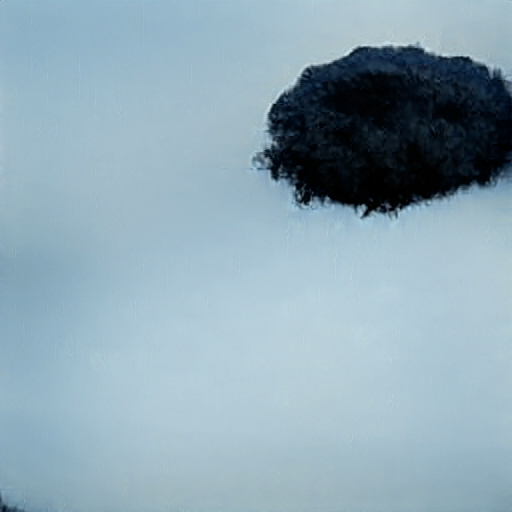
\includegraphics[width=.33\textwidth]{figures/c7_impact/other-artworks/offing/6.jpg}}
    \caption[Stills from \textit{The Offing}]{Stills from \textit{The Offing} \citep{sykes2022offing}. Images courtesy of Jen Sykes.}
    \label{fig:c7:offing}
 \end{figure}

\subsection{Derrick Schultz's \textit{You Are Here}}
\label{c7:subsubsec:schultz}

Derrick Schultz is an artist, designer and educator based in Brooklyn, New York. Schultz teaches at the Interactive Telecommunications Program at the New York University Tisch School of the Arts, and online under his own range of popular online courses for making AI art called Artificial Images. 
Schultz has used network bending in a number of his own artworks and has even produced tutorials showing others how to use it \citep{schultz2020netbending}. 

To create the video work \textit{You Are Here}, \citep{schutlz2020you} combined network bending with other machine-based forms of image manipulation and processing to produce original results divergent from any original training data, in a process that I described as `model chaining' in the active divergence taxonomy (\S \ref{survey:chaining}).
Schultz uses a custom StyleGAN2 model trained on illustrations of flowers and renders from latent interpolation. 
While rendering Schultz applied network bending transformations to add rotation to the image and have that processing in real-time. 
That image is then fed into an image translation model (BigBiGAN) \citep{donahue2019large} to get a different, further divergent image (Fig. \ref{fig:c7:you-are-here} for a visual representation of this process). 
The final machine learning step Schultz uses is SuperSlowMo \citep{jiang2018super} to interpolate frames in the original sequence to extend the duration to 1000x the original duration.

\begin{figure}[!htb]
    \centering
    \captionsetup{justification=centering}
    \includegraphics[width=1\textwidth]{figures/c7_impact/other-artworks/you-are-here.png}
    \caption[Example of the process behind making \textit{You Are Here}]{Example of the process behind making \textit{You Are Here} \citep{schutlz2020you}. Left: custom trained StyleGAN2 model. Middle: network bending rotation on StyleGAN Model. Right: BigBiGAN reinterpretation of output after network bending. Images courtesy of Derrick Schultz.}
    \label{fig:c7:you-are-here}
\end{figure}

For Schultz, using this esoteric and complex chain of computational models was a way to separate himself from other AI artists who were training StyleGAN models on similar datasets, and create results that could not be produced with a generative model designed to imitate a single dataset. 
A further discussion of how Schultz uses network bending, in combination with other generative models and image translation techniques is given in \S \ref{survey:chaining}.

\subsection{Hans Brouwer's \textit{Ouroboromorphism}}

\textit{Ouroboromorphism} \citep{brouwer2020ourobo}  (Fig. \ref{fig:c7:ouroboromorphism}) is an audiovisual work made by Hans Brouwer, an artist and researcher working towards his Masters degree at the Delft University of Technology. 
This work was created as part of a broader investigation into developing audio-reactive StyleGAN latent interpolations \citep{brouwer2020audio}. 

\begin{figure}[!htb]
    \centering
    \captionsetup{justification=centering}
    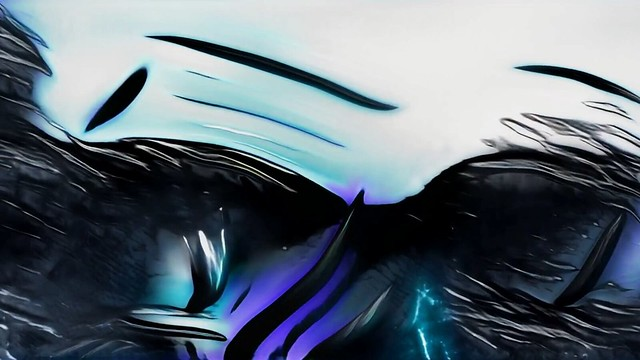
\includegraphics[width=1\textwidth]{figures/c7_impact/other-artworks/Ouroboromorphism.png}
    \caption[Still from \textit{Ouroboromorphism}]{Still from \textit{Ouroboromorphism} \citep{brouwer2020ourobo}. Image courtesy of Hans Brouwer.}
    \label{fig:c7:ouroboromorphism}
\end{figure}


Using a custom StyleGAN model, trained on abstract imagery that resembles abstract paintings and illustrations.
 Brouwer uses audio features to manipulate the latent vector codes for real-time generation. 
 In addition, he uses network bending transformations to add an additional level of control to support manipulating the visuals in response to audio, which would be possible with latent vector manipulation alone, which allows for `increasing the musical information that can be conveyed in a given period of time' \citep{brouwer2020audio}. 

Network bending was used in response to two sets of audio features that are recognised.
If kicks (sound resembling a kick drum) are found to be in the audio sequence, a zooming effect will be made to correspond to that sequence in time. If a snare (sound resembling a snare drum) is made, then a horizontal translation is made of the visuals. 
Brouwer also achieves a larger resolution and 2:1 aspect ratio by mirroring the activation maps in the earlier layer of the gan so that all of the generations are doubled with then onwards, in a similar manner to how I achieved the wider aspect ratio with \textit{Disembodied gaze} (\S \ref{c7:subsubsec:disembodied}) and \textit{Fragments of self} (\S \ref{c7:subsubsec:fragments}). 

In addition to network bending, Brouwer also adopted model rewriting \citep{bau2020rewriting} as an additional active divergence method that can be used to manipulate the visual representations (\S \ref{survey:rewriting}).

\section{Technical impact of Network Bending}
\label{c7:sec:net-bend-impact}

The experiments presented in Chapter \ref{ch:net_bend} have gone on to influence further technical development of network bending being applied to other kinds of generative models, the design of generative model architectures themselves, and have also been integrated into many user interface designs. All of these developments of network bending by others are detailed in the rest of this section.

 \subsection{Alias-Free GAN (aka StyleGAN3)}

 Alias-free GAN (later renamed StyleGAN3) by Kerras et al. (2021) was NVIDIA corporation's successor to their flagship StyleGAN1 and 2 neural networks. 
 The alias-free GAN approach was designed from the ground up to be fully equivariant to the transformation of their internal representations (aka network bending). 
 This architecture can produce internal features that are equivariant to either two kinds of transformation, translation or rotation. 

 One of the artefacts revealed when network bending was performed on StyleGAN2 models was the ‘texture sticking’ effect, which can be seen when animating a transformation, such as a translation or rotation, where the fine details are stuck to specific pixel coordinates. 
 The authors attributed the texture sticking to `unintentional positional references made to intermediate layers from the borders of the image, per-pixel noise inputs and aliasing between layers'. 
 The traditional network architecture `ha[ve] the means and motivation to amplify even the smallest amounts of aliasing and combine it over multiple scales to build a basis for texture motifs that are fixed in screen coordinate space' \citep{karras2021alias}.
 Reflecting on this, they make a major overhaul to the convolutional framework used in the generative model and replace the convolutional layers in the generator with pointwise convolutional layers.

 \begin{figure}[!htb]
    \centering
    \captionsetup{justification=centering}
    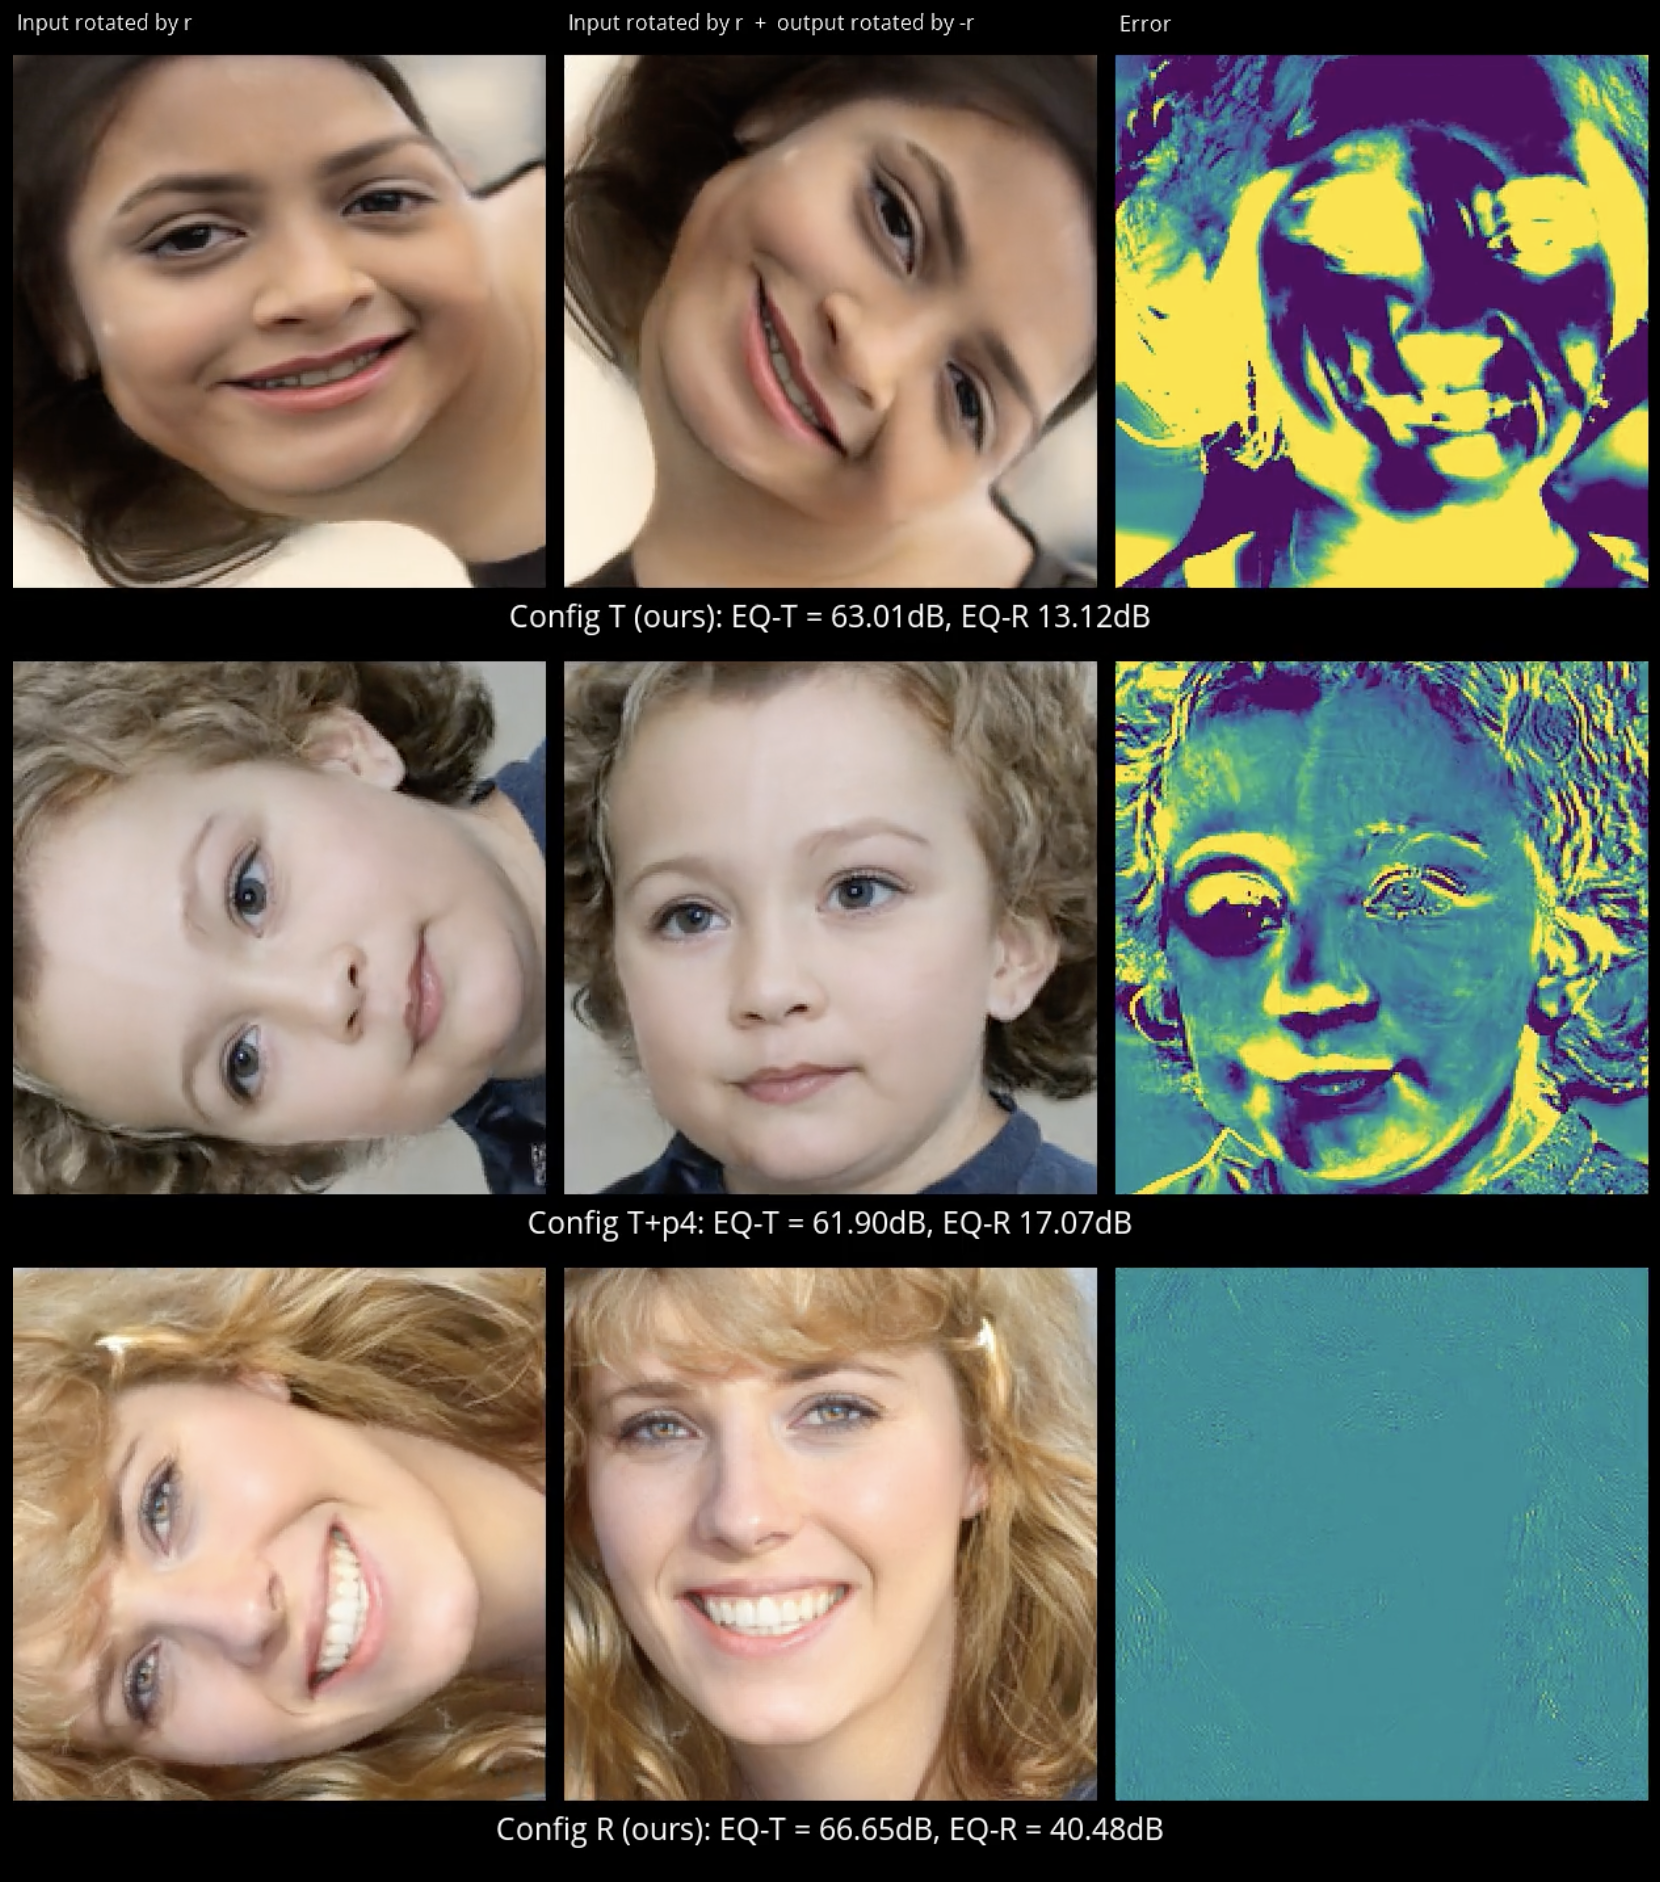
\includegraphics[width=1\textwidth]{figures/c7_impact/net-bend-technical/style-gan-rotations.png}
    \caption[Network bending in Alias-Free GAN (StyleGAN3)]{Network bending in Alias-Free GAN (StyleGAN3). \citep{karras2021alias}. Image reproduced under the Creative Commons CC BY-NC 4.0 licence.}
    \label{fig:c7:alias-free-gan}
\end{figure}

 The StyleGAN3 paper cites the original network bending paper from EvoMUSART \citep{broad2021network}.
 It is clear, from the direction of the research and its evaluation in the technical and public-facing demos that network bending has informed the advancement of the technical development work of the architecture of StyleGAN's development, as well as the evaluation of those improvements and how that is communicated publicly  (Fig. \ref{fig:c7:alias-free-gan}). 
 Having a network architecture that was better suited to manipulation of the internal representations of the model has, in their words, `pave[d] the way for generative models better suited for video and animation.' \citep{karras2021alias}.

StyleGAN3 was and largely still is the state-of-the-art in fidelity and controllability of GAN architectures. 
This went on to be superseded in terms of fidelity and flexibility of image generation by diffusion-based models, particularly, latent diffusion \citep{rombach2022high} which is very intuitive and flexible to control with text-to-image conditioning.
At the time of writing StyleGAN3 is still one of the leading architectures for feed-forward image generation, with network bending being core to the development of its improvements on StyleGAN2. 

\subsection{Interfaces Developed for Network Bending}
\label{c7:subsec:net-bend-interfaces}

Building an interface was something that I had originally planned as follow-on work from the original network bending paper in 2020. 
Unfortunately, illness and other restrictions from the pandemic impeded my ability to do that. 
However, in the intervening time many other people have developed their own interfaces for network bending for both image and audio generation.

\subsubsection{StyleGAN3 Visualiser}

In the release of the StyleGAN3 codebase on GitHub, NVIDIA corporation built and provided a user interface for interactively generating samples, visualising internal feature representations, and applying the x-y translation and rotation transformations  (Fig. \ref{fig:c7:stylegan3-interface}).  

\begin{figure}[!htb]
    \centering
    \captionsetup{justification=centering}
    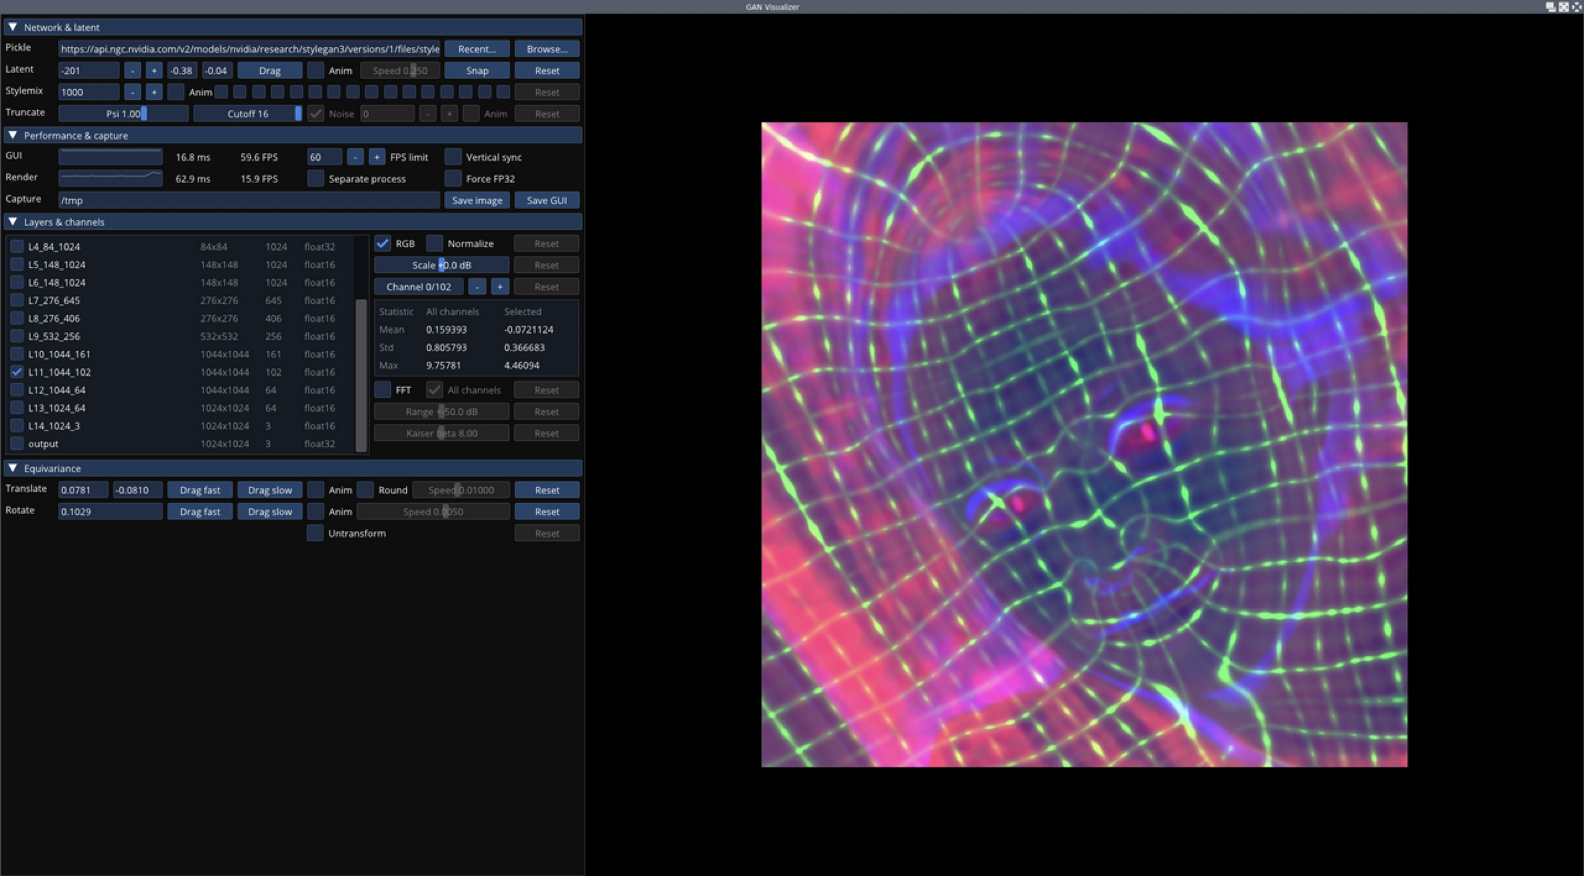
\includegraphics[width=1\textwidth]{figures/c7_impact/net-bend-technical/stylegan3-vis-interface.png}
    \caption[StyleGAN3 user interface]{Screenshot of StyleGAN3 user interface \citep{karras2021alias}. Image reproduced under the Creative Commons CC BY-NC 4.0 licence.}
    \label{fig:c7:stylegan3-interface}
\end{figure}


These translations are only applied layer-wide, but the code is configured such that animations of these transformations being applied with linearly changing parameters can be applied. 

\subsubsection{Autolume}

In the AutoLume-live system, \citep{kraasch2022autolume,kraasch2023autolume} network bending is one of several features integrated into a real-time GAN-based VJing (Video Jockey) system. 
The latent vectors are determined by musical features amplitude, pitch and onset strength. 
These audio features create latent trajectories for the animation created with the GAN. 
A GUI (Graphical User Interface) which can also be controlled by MIDI (Musical Instrument Digital Interface) is developed to allow the user to improvise and adjust this generative process in real time, with network bending transformations being one of the manipulations that can be made  (Fig. \ref{fig:c7:autolume-live}). 
Autolume can be operated using a physical mixing desk interface using MIDI.

\begin{figure}[!htb]
    \centering
    \captionsetup{justification=centering}
    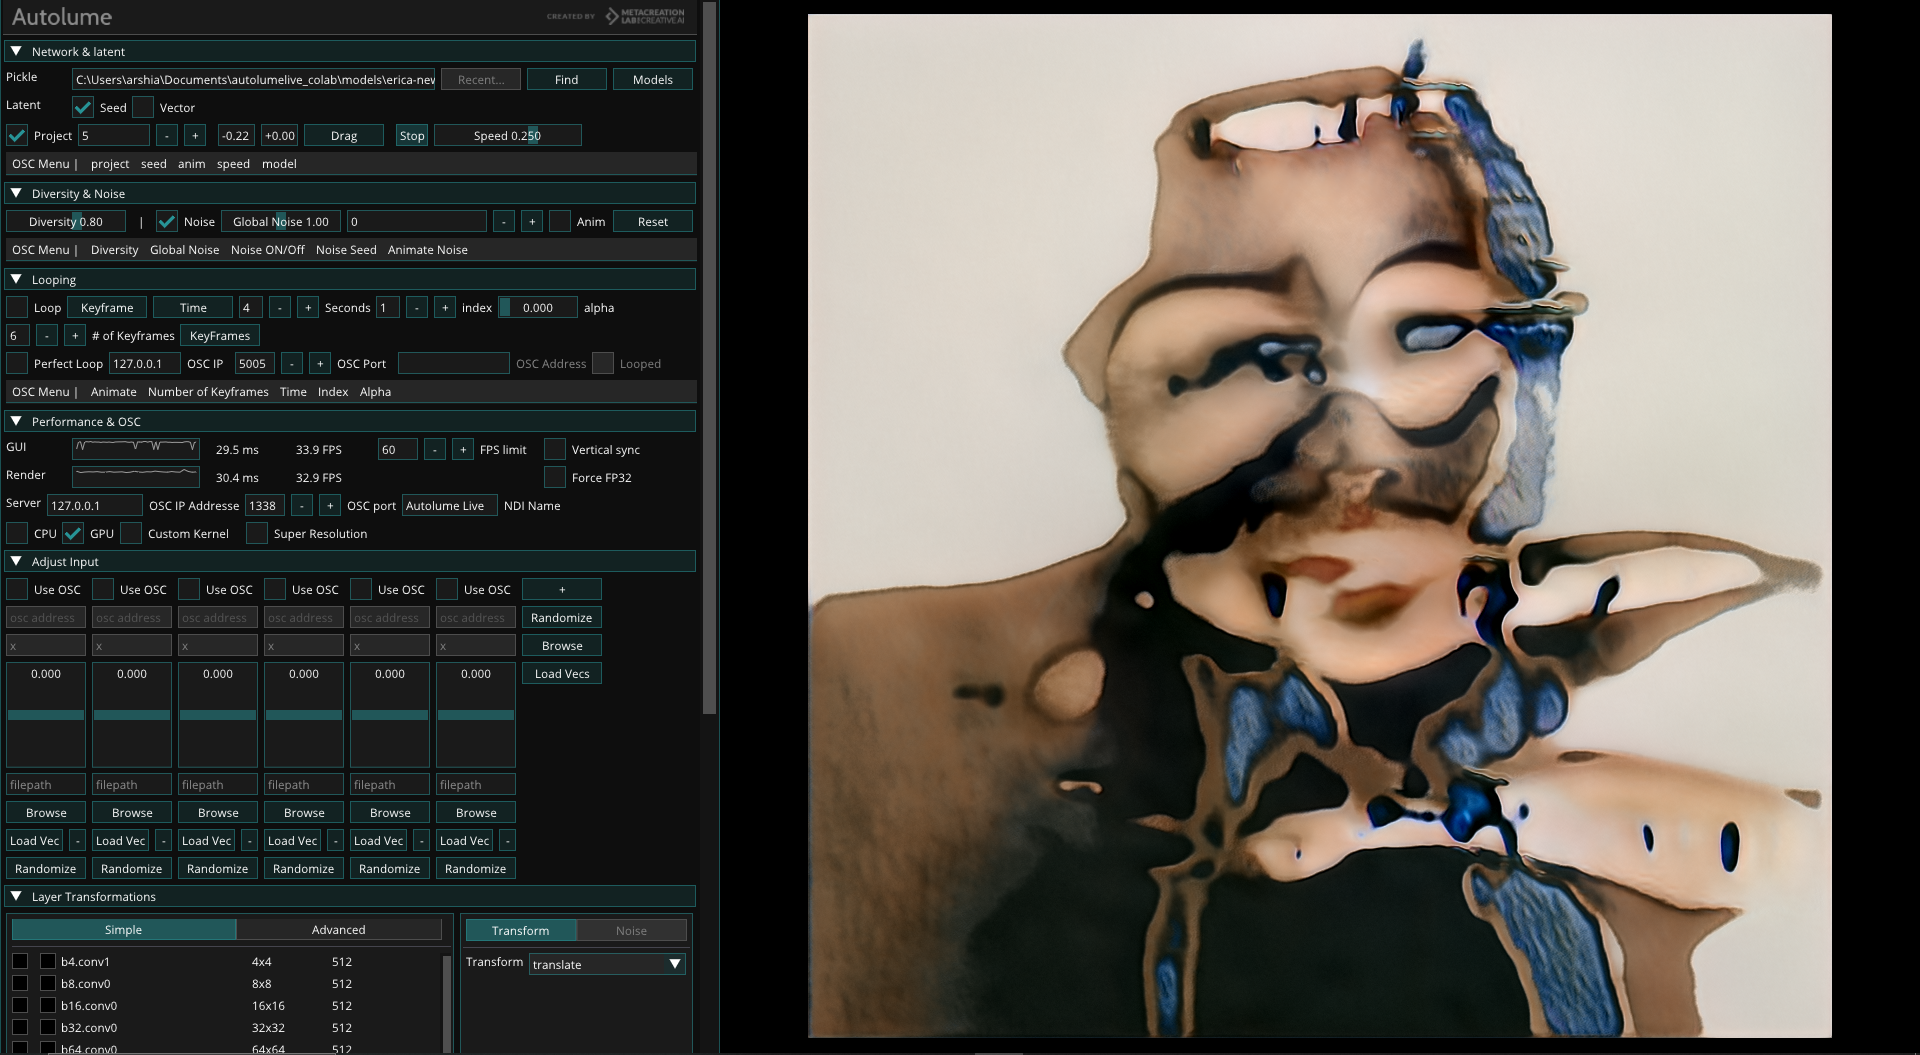
\includegraphics[width=1\textwidth]{figures/c7_impact/net-bend-technical/autolume-live.png}
    \caption[Autolume-live user interface]{Screenshot of Autolume-live user interface \citep{kraasch2023autolume}. Image courtesy of Jonas Kraasch.}
    \label{fig:c7:autolume-live}
\end{figure}

\subsubsection{StyleGAN-Canvas}

StyleGAN-Canvas is a mixed-initiative interface \citep{zheng2023stylegan}, combining image-to-image translation with rendering performed by StyleGAN3. 
A custom encoder was trained to perform image to latent real-time encoding, allowing users to take webcam or other input images and use that as the starting point for GAN rendering  (Fig. \ref{fig:c7:stylegan-canvas}). 
Parameters for controlling network bending transformations: erosion, dilation, pointwise scalar multiplication, x-y translations, rotation, and scaling.
The clustering algorithm described in the previous chapter has also been implemented and clusters for StyleGAN3 models were calculated and integrated into the interface.

\begin{figure}[!htb]
    \centering
    \captionsetup{justification=centering}
    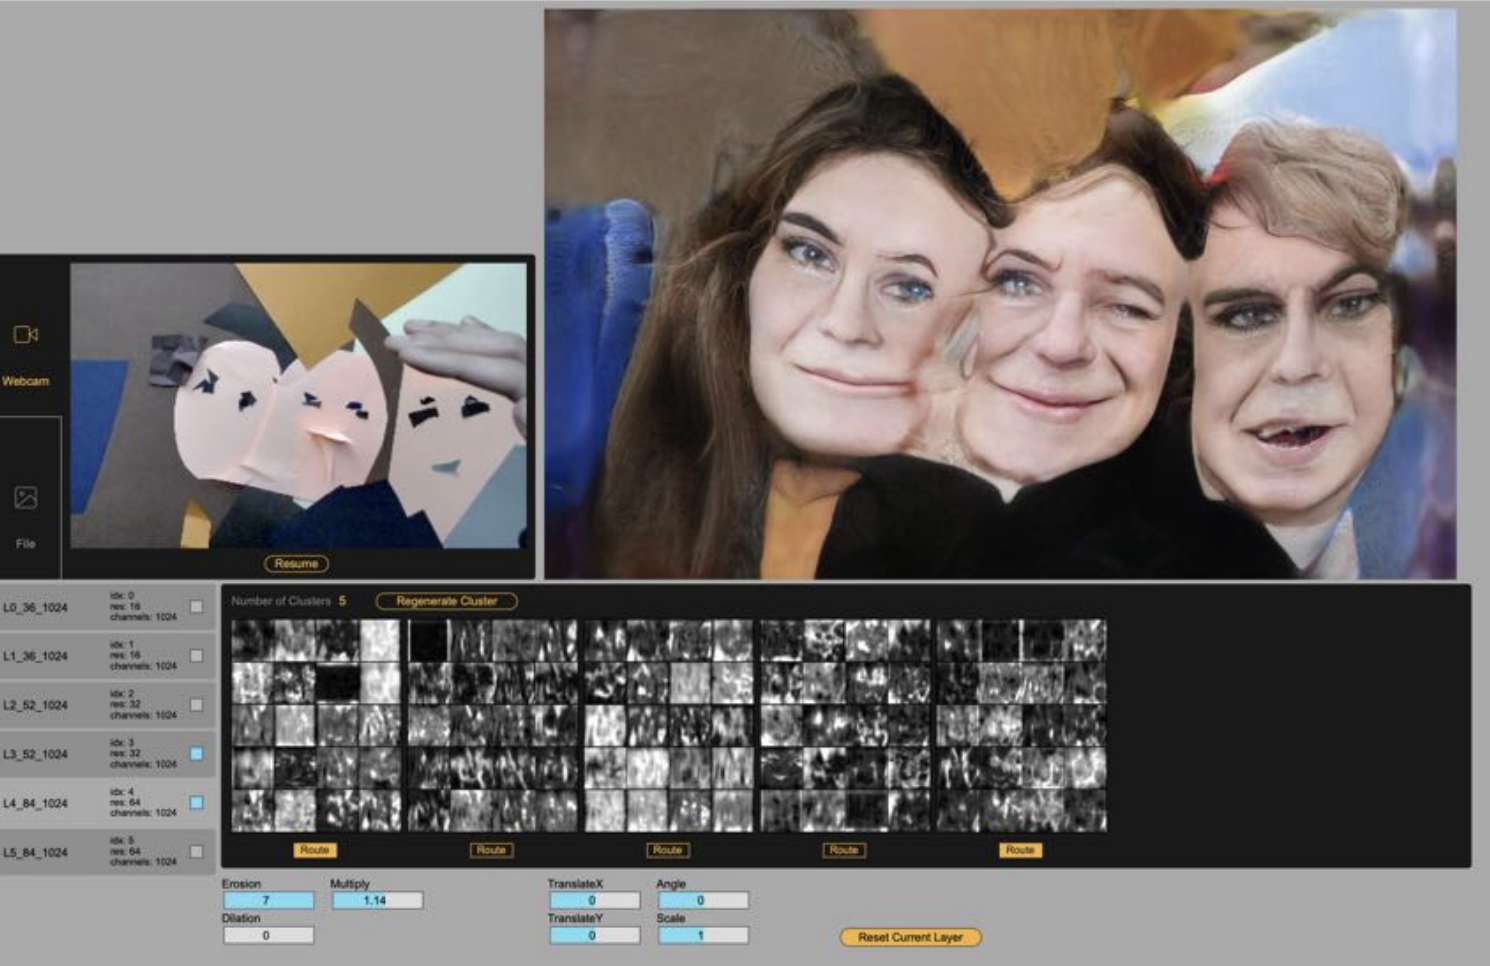
\includegraphics[width=1\textwidth]{figures/c7_impact/net-bend-technical/stylegan-canvas.png}
    \caption[StyleGAN-Canvas user interface]{Screenshot of StyleGAN-Canvas user interface \citep{zheng2023stylegan}. Image courtesy of Shouyang Zheng.}
    \label{fig:c7:stylegan-canvas}
\end{figure}

\subsubsection{Network Bending Audio Inteface}
\label{c7:subsubsec:naotokui}

The musician and researcher Nao Tokui built his own user interface applying Network Bending to audio \cite{tokui2023bending}. 
This was done using a StyleGAN model trained on spectrograms, in a similar fashion to \S \ref{c5:sec:net-bend-audio}.
This user interface was designed for real-time performance, where the transformations are applied in real-time to a model generating spectrograms, the output of which is being looped for real-time musical performance  (Fig. \ref{fig:c7:net-bend-nao-tokui}).

\begin{figure}[!htb]
    \centering
    \captionsetup{justification=centering}
    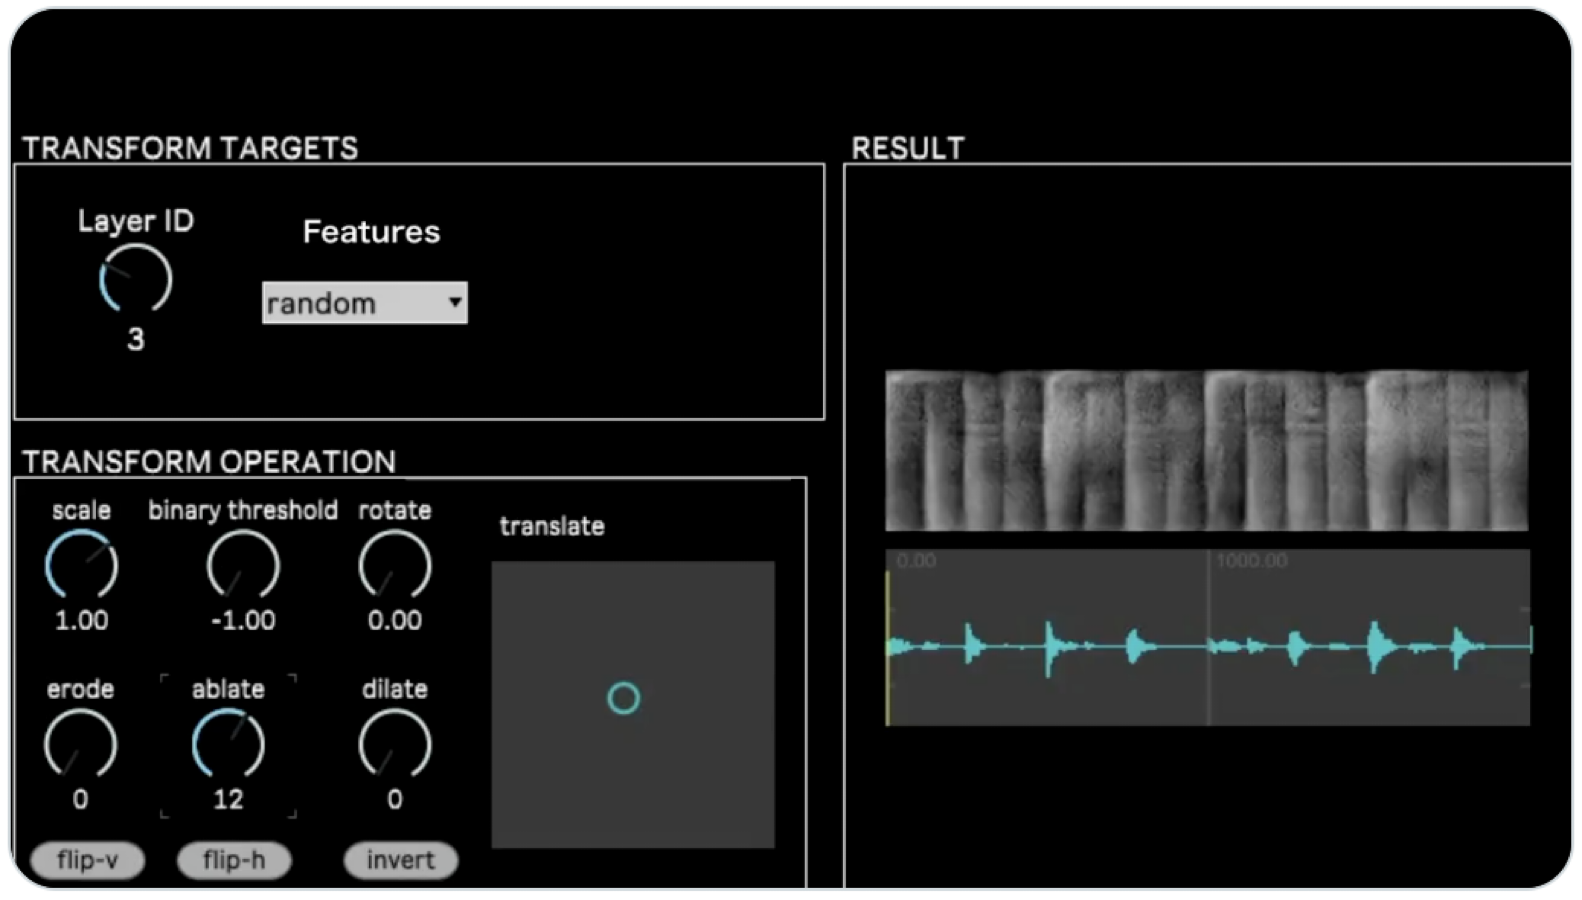
\includegraphics[width=1\textwidth]{figures/c7_impact/net-bend-technical/nao-tokui-stylegan-audio.png}
    \caption[Network bending audio user interface]{Screenshot of Network bending audio user interface \citep{tokui2023bending}. Image courtesy of Nao Tokui.}
    \label{fig:c7:net-bend-nao-tokui}
\end{figure}

\section{Further Advancements of Network Bending}

Network bending was originally built to be run in feedforward generative models that use a convolutional architecture, like GANs or VAEs. 
However, the principal can be applied to other architecture of generative models and does not need to even use the paradigm of deterministically controlled filters. 
The rest of this section details extensions of network bending beyond the original paradigm described in Chapter \ref{ch:net_bend}.

\subsection{Network Bending DDSP}
\label{c7:subsubsec:ddsp}


The first extension of network bending was undertaken by Matthew Yee-king and Louis McCallum \citep{mccallum2020network,yee2021studio}. 
In this work, they took the Differential Digital Signal Processing model (DDSP) from Google Magenta, which is a neural network for audio synthesis and manipulation for tasks such as timbre transfer. 
The DDSP model takes frequency and amplitude values and it outputs 101 control values for an oscillator and noise filter parameters. 
In the network bending DDSP framework, network bending transformations are applied to the three layers in the neural network where all of the features are combined. 
There are four different types of transformation in this work: ablate, invert and binary threshold have been kept from the work described in the last chapter.
 In addition, Yee-king and McCallum implemented an oscillate transformation that performs a sin wave transformation based on the frequency and the depth of the layer in the network. 

 \subsection{Network Bending Diffusion Models}
 \label{c7:subsec:netbend-diffusion}

 \cite{dzwonczyk2024network} apply the standard approach of network bending to denoising diffusion generative models  (Fig. \ref{fig:c7:net-bend-diffusion}).
 In this work, they apply the same point-wise, affine and morphological transformations as described in \S \ref{c5:sec:transforms} to convolutional activation maps in the U-Net model \citep{ronneberger2015u} that is used in latent diffusion models \citep{rombach2022high}. 
 Latent diffusion models can be conditioned on text, to perform text-to-image generation.
 By using network bending in the text-to-image pipeline, it is shown that altering the features can cause semantic shifts to occur between concepts, depending on the network bending parameters used.

\begin{figure}[!htb]
    \centering
    \captionsetup{justification=centering}
    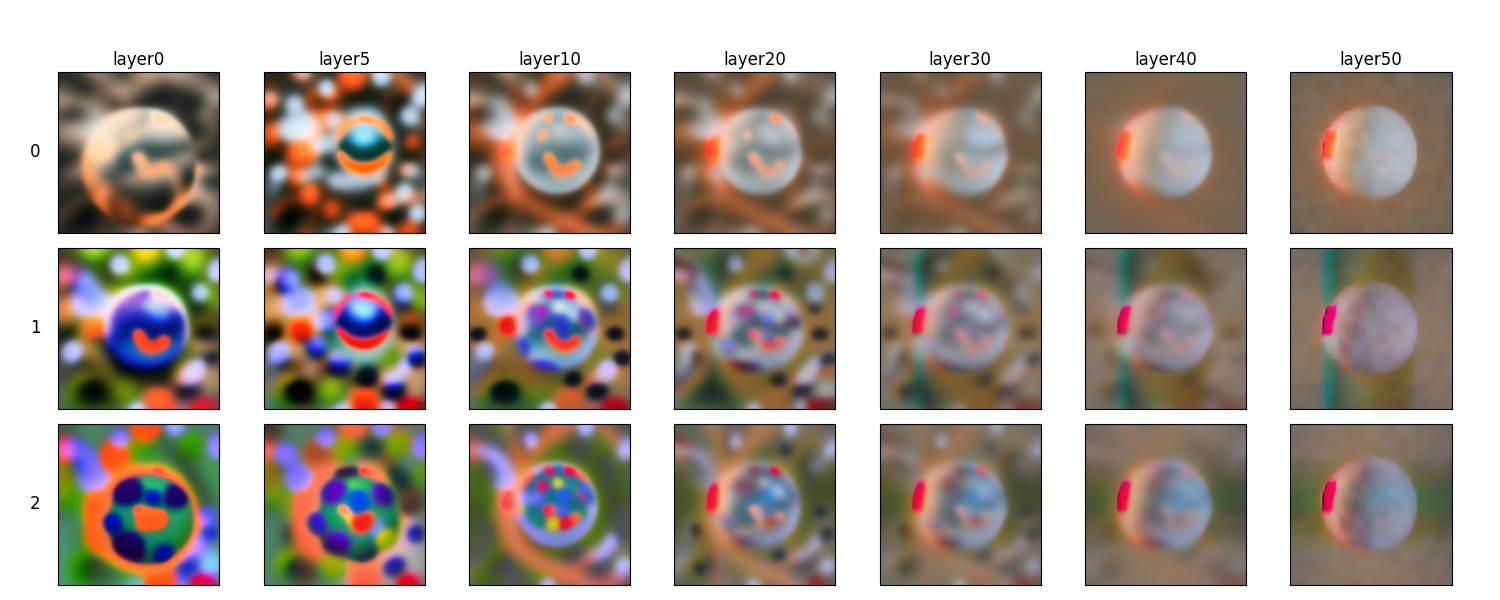
\includegraphics[width=1\textwidth]{figures/c7_impact/net-bend-technical/net-bend-diffusion.png}
    \caption[Network bending in diffusion models]{Network bending in diffusion models \citep{dzwonczyk2024network}. Applying erosion with normalization at different layers to the prompt `a floating orb'. Each column shows normalization happening across a different dimension. Image courtesy of the Luke Dzwonczyk.}
    \label{fig:c7:net-bend-diffusion}
\end{figure}

\subsection{Differentiable Network Bending}

In differentiable network bending, \cite{aldegheri2023hacking} extend the concept of network bending from inserting deterministically controlled filters into models, to inserting additional modules into models that can be trained using gradient descent optimisation.
In the work, they insert additional layers into pre-trained GANs that transform the activation maps of all of the convolutional filters in a layer.
They optimise the weights of this new layer using CLIP \citep{radford2021learning} towards matching a pre-set text prompt  (Fig. \ref{fig:c7:differential-net-bend}).
In the paper, they note that using CLIP to optimise text prompts is just one possible way that this kind of system could be optimised. 

\begin{figure}[!htb]
    \centering
    \captionsetup{justification=centering}
    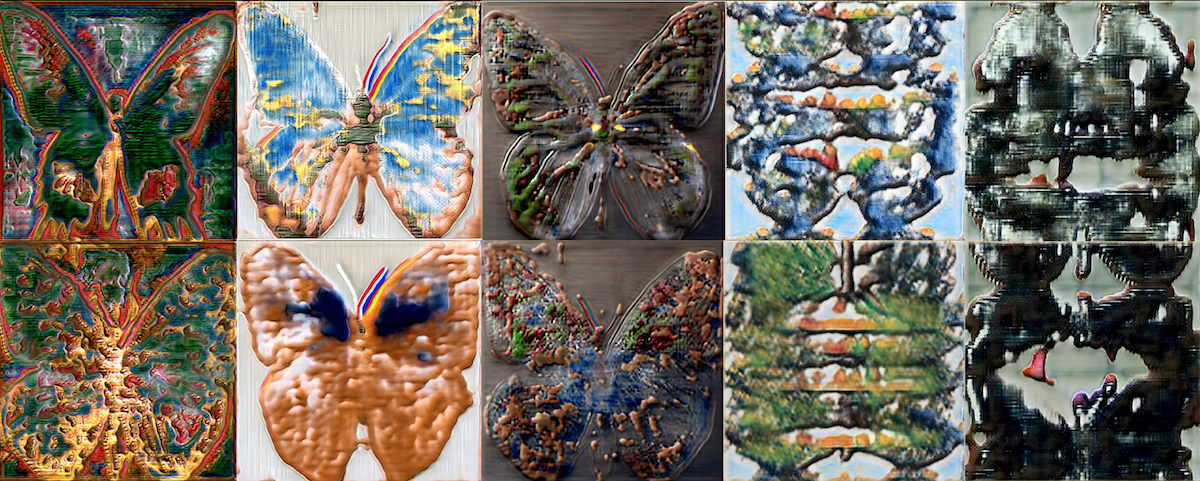
\includegraphics[width=1\textwidth]{figures/c7_impact/net-bend-technical/diff-net-bend.png}
    \caption[Differential network bending]{Examples of differentiable network bending \citep{aldegheri2023hacking} applied to a GAN model trained on butterflies, with the differential network bending model trained to optimise various text prompts. Image courtesy of Giacomo Aldegheri.}
    \label{fig:c7:differential-net-bend}
\end{figure}


\section{Conclusion}

This chapter has detailed the impact the experimental work in my PhD has had, in both the cultural and technical sectors. 
This includes detailing the artworks made by myself and other practitioners, and the work done to extend and build interfaces to interact with the work I have developed. 
In particular, the network bending framework has been the work that has been most adopted by others. 
In all these cases, network bending has been adapted to allow for further generative possibilities that were available with traditional training of generative models. 
Referring back to the title of this thesis, \textit{Expanding the generative space}, it is this piece of work that has most successfully had an impact in that regard. 

The next chapter will reflect on the technical contributions of this thesis, as well as the impact it has had and the broader developments that have happened in the field during the course of my work on this PhD.
